\documentclass[a4paper,12pt]{article}
\usepackage{fontspec}
\usepackage[utf8]{inputenc}
\usepackage{graphicx}
\usepackage{ragged2e}
\usepackage{import}
\usepackage{geometry}
\usepackage[export]{adjustbox}
\usepackage{multicol}
\usepackage{setspace}
\usepackage{lipsum}  
\usepackage{hyperref}
\usepackage{indentfirst}
\usepackage{lettrine}
\usepackage{float}
\usepackage{caption}
\usepackage{graphicx}
\usepackage{pdfpages}
\usepackage{parskip}




\special{pdf:minorversion 7} %set minorversion




\title{Rapport Project fin d'études SPN Cars mobile App}
\author{Alaa Abdelbaki}
\date{2022}

\graphicspath{{./images/}}
\setmainfont{Times New Roman}
\onehalfspacing
\renewcommand*\contentsname{Table de matières}
\renewcommand*\listfigurename{Liste de figures}





\begin{document}
% Title page
% \thispagestyle{empty}
\graphicspath{{./images/}}
\newgeometry{top=1cm,bottom=1cm}

\justifying
\centering

% \begin{multicols}{2}
%    
\includegraphics[width=0.25\textwidth,left]{esprit.jpg}
%    
\includegraphics[width=0.25\textwidth,right]{spn_logo.png}
% \end{multicols}
\centering
\textbf{{\footnotesize République Tunisienne}}\\
\textbf{{\footnotesize Ministère de l'enseignement supérieur, de la recherche scientifique et de la technologie}}\\
\textbf{{\footnotesize Institut Supérieur Privé d'Ingénierie et de Technologies}}\\
\bigbreak

\includegraphics[width=0.5\linewidth]{esprit.jpg} \\
\bigbreak
\textbf{{\huge Rapport de stage de fin d'études}} \\
\bigbreak
\bigbreak
\bigbreak
{\large Présenté en vue de l'obtention du} \\
\bigbreak
{\large Diplôme National d'Ingénieur en Informatiques} \\
\bigbreak
\textbf{{\large Option:}}\\
\bigbreak
{\large Systèmes Informatiques et Mobiles}
\bigbreak
\bigbreak
\bigbreak
{\large Sujet:}\\
\bigbreak
\textbf{{\Large << Conception, développement et mise en place de l'application mobile SPN Cars >>}}
\bigbreak
\bigbreak
\bigbreak
{\large Elaboré par :}\\
\bigbreak
\textbf{{\large Alaa Abdelbaki}}
\bigbreak
\bigbreak
{\large Au sein de :}
\bigbreak

\includegraphics[width=0.5\linewidth]{spn_logo.png}
\bigbreak
\begin{multicols}{2}
    \centering
    Encadrant Swiss Premium Negoce\\ \textbf{Mr. Ghaith BEN ABDESSALEM}
    Encadrant ESPRIT\\ \textbf{Mme. Nouha Samet}
\end{multicols}
\vspace*{\fill}
\textbf{\footnotesize Année universitaire: 2021/2022}
\newpage
\thispagestyle{empty}
\
\newpage






\includepdf[pages={1}]{./chapters/garde.pdf}
\newpage
\thispagestyle{empty}
\mbox{}\\
% Dédicaces
\raggedright
\newpage
\newgeometry{margin=2.5cm}

% Remerciements
\newpage
\thispagestyle{empty}
\newgeometry{left=4cm,right=2.5cm}
\begin{center}
    \begin{huge}
        \textbf{Remerciements}
    \end{huge}
\end{center}
\vspace{2cm}
\begin{small}
    \justifying


    Au terme de ce projet, je tiens à adresser mes remerciements les plus sincères et à exprimer ma gratitude envers mon encadrant pédagogique Madame Nouha Samet dont l'assistance et la disponibilité étaient présentes tout au long du stage.


    Je la remercie aussi pour ses directives et els conseils qu'elle m'a prodiguée pour atteindre les objectifs du stage dans les délais convenus.
    Je dois aussi une grande partie de mon travail à Monsieur Ghaith Ben Abdessalem. Je le remercie pour pour sa disponibilité, ses remarques constructives qui m'ont aidé à surmonter beaucoup de difficultés et à améliorer les fonctionnalités de l'application ainsi que ses qualités humaines d'écoute et de compréhension tout au long de ce travail.


    J'exprime également ma gratitude envers tous les membres de la société Swiss Premium Negoce qui m'ont apporté leur soutien et leur savoir faire. J'ai découvert dans ce service une équipe jeune, dynamique et conviviale qui est devenue, pour moi, une famille. Je remercie également la directrice de département IT de la société Madame Jihene Ben Abderrazzek pour sa disponibilité et ses conseils qui ont été très bénéfiques tout au long de ce stage.


    Je tiens également à remercier tous les enseignants qui ont participé à mon évolution scientifique durant ses quatres années que j'ai passé au sein de ESPRIT. Je remercie finalement les membres du jury en espérant qu'ils apprécient ce rapport.
\end{small} \\
\bigbreak
\begin{flushright}
    \textbf{\textit{Alaa Abdelbaki}}
\end{flushright}
% Table of contents
\newpage
\tableofcontents
\newpage
\listoffigures
\newpage
% Introduction
\thispagestyle{plain}
\newgeometry{left=4cm,bottom=2.5cm}
\setcounter{page}{1}
\chapter*{Introduction générale}
\markboth{Introduction générale}{}
\addcontentsline{toc}{chapter}{Introduction générale}
\vspace{1cm}
\setlength{\parindent}{40pt}
\justifying
\begin{small}
    \lettrine[findent=2pt,lines=3]{\textit{L}}{}e marché mondial de location de voitures continue, chaque année, à se développer et à s'amplifier, et le besoin d'atteindre un nombre maximal de clients est devenu une nécessité. Surtout avec l'avancement technologique qui a permis a tous le monde d'avoir un smarthphone. Cet appareil capable de réaliser plusieurs fonctionnalités en simples clics.

    \noindent Pendant les années précédentes, avec la pandémie mondiale de COVID-19, qui a forcé des milliards de personnes à rester chez eux, il est devenu indispensable de digitaliser plusieurs services afin de les rendre plus accessible, plus fiable, et continuer à exister dans un marché qui continue à évoluer et innover. Plusieurs personnes on pû se bénéficier de ses services sans quitter leurs maisons et risquer être atteints par la COVID, grâce aux différentes entreprises qui ont choisi de continuer à servir leurs clients à l'aide des applications mobiles.

    \noindent L'entreprise Swiss Premium Negoce a vu cet évênement mondial comme une opportunité pour s'introduire dans le monde vaste de nouvelles technologies et présenter leurs différents servies sous forme numérique à l'aide des sites web et applications mobiles. Cette étape qui les permettra de rester toujours proche de sa clientèle, et continuer à fonctionner sans tenir compte de la pandémie.

    \noindent L'un des services offerts par Swiss Premium Negoce est le service de location de voitures de luxe. Ce service permet aux utilisateurs de trouver leurs voitures de rêves et la louer même pour une courte durée avec la possibilité d'avoir un chauffeur personnel. tout cela sera possible à l'aide de l'application Swiss Premium Negoce : Cars ou tout simplement : SPN Cars. Le présent rapport qui présentera cette application, s'étalera sur quatre chapitres:

    \begin{itemize}
        \item Le premier chapitre présentera l'organisme d'accueil, ainsi le projet à réaliser et une étude sur les différents aspects de ce projet.
        \item Le deuxième chapitre fera l'objet de présenter les différents besoins qui seront achevés par cette application.
        \item Le troisième chapitre sera à propos la conception de l'application, et les technologies choisies pour réaliser le projet suite à cette application.
        \item Le quatrième et dernier chapitre présentera la réalisation de ce projet, qui est une explication détaillée de chacune des fonctionnalités offerts par l'application avec des captures d'écran pour illustrer le travail réalisé.
    \end{itemize}

    \noindent Le projet sera clôturé par une conclusion générale.
\end{small}
\newpage
% Cadre du projet
\newgeometry{margin=2.5cm}
\section{Cadre du projet}
% \subsection{Introduction}
\small{\textit{Vu que ce projet de fin d'études sera réalisé au sein d'une entreprise accueillante, il s'avère être indispensable d'avoir une idée sur cette dernière. Par suite, nous allons mettre l'accent sur le sujet et les motivations derrière ce projet.}}
\subsection{Présentation de l'organisme d'accueil}
Ce projet a été réalisé au sein du tout nouveau département IT de \textit{\textbf{Swiss Premium Negoce}}.\\
\noindent Ce département ce compose d'une équipe très innovante, très talentueuse qui est responsable des différents applications et sites web de tous les différents services proposés par SPN.
\subsubsection{Présentation générale}
\vspace{1cm}
\begin{figure}[H]
    \centering
    
\includegraphics[width=0.25\textwidth]{spn_logo.png}
    \vspace{0.5cm}
    \caption{Logo Swiss Premium Negoce}
    \label{fig:spn_logo}
\end{figure}
\vspace{1cm}
\textit{\textbf{Swiss Premium Negoce SA}} (Société Anonyme) est une société de conciergerie basée à Genève, Suisse.\\
\noindent 'Créée en 2011 avec passion et enthousiasme, l'ntreprise se spécialise en services de luxe.
En 2022, SPN a inauguré son nouveau département IT, un département qui permettera d'atteindre plus d'audience grâce à la digitalisation des plusieurs services offerts par SPN.
\subsubsection{Activitées}
SPN offre plusieurs services de luxe tel que:
\begin{itemize}
    \item Conciergerie
    \item Hospitalité de luxe
    \item Location de voitures
    \item Santé et services médicaux
    \item Camps d'été
    \item Éducation
    \item Jets privés
    \item Yachting
\end{itemize}
\subsection{Présentation du projet}
\subsubsection{Présentation générale}
L'application SPN-Cars est la solution trouvée par SPN pour offrir l'un de ses services les plus demandés plus facilement et convenablement grâce à l'utilisation de plusieurs nouvelles technologies qui permetteront à l'entreprise de mieux performet at atteindre plus d'utilisateurs.\\
\noindent On doit alors définir ce projet, son objectif, ses concurrents, les problèmes qu'ils créent et comment l'application SPN-Cars pourra les corriger et offrir un service meilleur que les autres applications disponibles sur le marché.
\subsubsection{Problématique}
L'appliaction SPN-Cars vise à devenir l'un des leaders dans les domaines de location de voiture en ligne, réservation de chauffeurs et des services taxis. Ce qui pose un grand défi : \textbf{Comment fournir aux utilisateurs de l'application ses services en tenant compte de la rapidité de l'application ainsi que la facilité des procédure ?}
\subsubsection{Etude de l'existant}
Il existe déjà plusieurs applications qui offrent des services similaires, chacune de ses applications présente des avantages et des inconvénients qu'on les explorera dans les chapitres suivants.
\phantomsection
\paragraph{Sixt}\mbox{} \\
\vspace{1cm}
\begin{figure}[H]
    \centering
    
\includegraphics[width=0.25\textwidth]{sixt.png}
    \vspace{0.5cm}
    \caption{Logo Sixt}
    \label{fig:sixt_logo}
\end{figure}
\vspace{1cm}
Sixt est in fournisseur international de voitures de location, avec plus de 2000 véhicules dans 110 différents pays.\\
\noindent Sixt offre plusieurs services en rapport avec la location des voitures :
\begin{itemize}
    \item Location des voitures.
    \item Covoiturage.
    \item Service taxi.
    \item Location de voiture par abonnement mensuel.
\end{itemize}
\paragraph{Blacklane}\mbox{} \\
\vspace{1cm}
\begin{figure}[H]
    \centering
    
\includegraphics[width=0.25\textwidth]{blacklane.jpg}
    \vspace{0.5cm}
    \caption{Logo Blacklane}
    \label{fig:blacklane_logo}
\end{figure}
\vspace{1cm}
Blacklane est une entreprise allemande qui offre à ses clients la possiblité de réserver un chauffeur avec une voiture luxueuse et vivre une expérience VIP.\\
\noindent L'entreprise offre principalement trois services :
\begin{itemize}
    \item Tragets longue distance.
    \item Chauffeurs à la demande.
    \item Transfert aéroport.
\end{itemize}
\paragraph{Uber}\mbox{} \\
\vspace{1cm}
\begin{figure}[H]
    \centering
    
\includegraphics[width=0.25\textwidth]{uber.jpg}
    \vspace{0.5cm}
    \caption{Logo Uber}
    \label{fig:uber_logo}
\end{figure}
\vspace{1cm}
Uber est une entreprise de technologies américaine qui propose à ses clients une solution de trouver des chauffeurs pour les transporter vers leurs destination choisie grâce à son application mobile.\\
\noindent Uber a commencé en tant qu'une application qui joue le rôle d'intermédiaire entre ses utilisateurs et ses chauffeurs indépendants qui offrent leurs services.
\subsubsection{Critique de l'existant}
Même si les exemples mentionnés ci-dessus sont les leaders mondiaux dans le domaine de services de transport, ils sont tous différents. Surtout en terme de qualité de services, du marché visé.\\
\noindent Uber, par exemple, est à la recherche d'attirer un nombre maximal d'utilisateurs, c'est pourquoi l'application offre une sélection très variée de moyens de transport (voire fig. 5). Blacklane, par contre, vise une clientèle plus exclusive, une clientèle qui est prête à payer pour avoir un service de luxe. Ce qui est visible lors de la sélection de voitures à l'aide de l'appliction Blacklane comme le montre la figure ci-dessous (voir fig. 6)
\vspace{1cm}
\begin{multicols}{2}
    \begin{figure}[H]
        \centering
        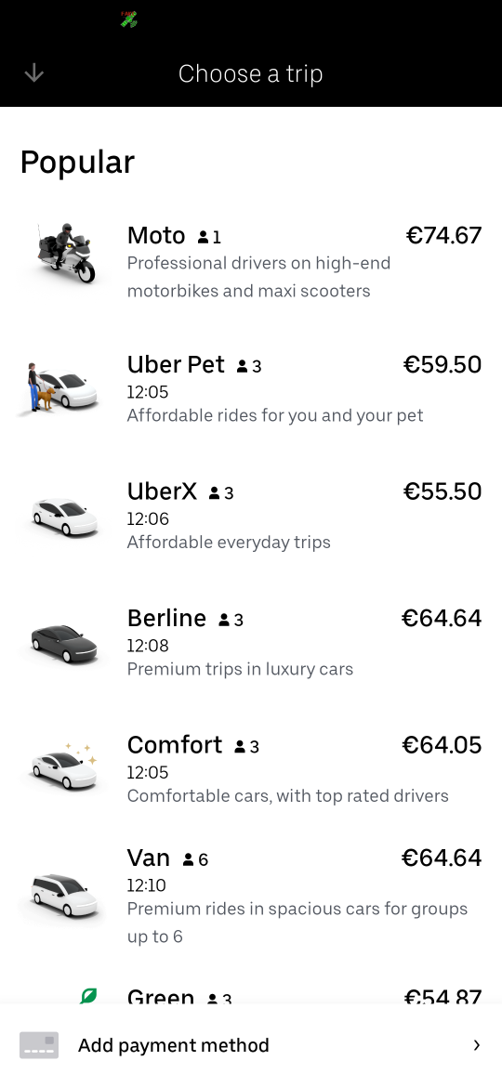
\includegraphics[height=0.5\textheight]{uber-car-selection.png}
        \vspace{1cm}
        \caption{Sélection de voiture avec Uber}
        \label{fig:uber_selection}
    \end{figure}
    \begin{figure}[H]
        \centering
        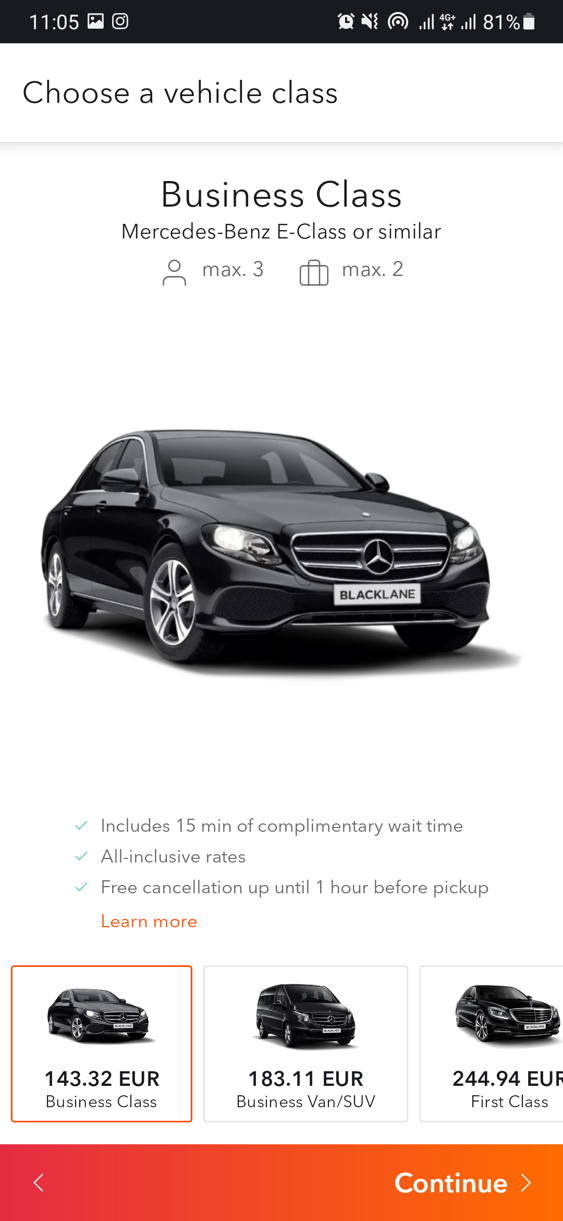
\includegraphics[height=0.5\textheight]{blacklane-car-selection.png}
        \vspace{1cm}
        \caption{Sélection de voiture avec Blacklane}
        \label{fig:blacklane_selection}
    \end{figure}
\end{multicols}
\subsubsection{Solution Proposée}
% TODO : FInish this section
L'objectif de l'application SPN-Cars est de fournir à ses utilisateurs des expériences luxieuses en simples clics.\\
L'application doit avoir un
\begin{figure}[H]
    \centering
    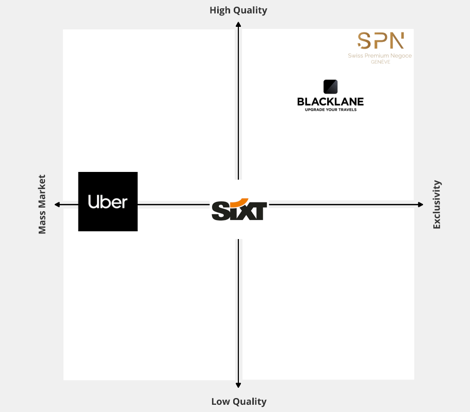
\includegraphics[height=0.5\textheight]{positionnement.png}
    \vspace{1cm}
    \caption{Positionnement de l'application SPN-Cars par rapport aux alternatives.}
    \label{fig:positionnement_marcha}
\end{figure}

% Spécifications des besoins
\newpage
\chapter{Spécification des besoins}
\minitoc
\clearpage
\section*{Introfuction}
L'application \textbf{SPN-Cars} est une application mobile permettant à ses utilisateurs de louer des voitures luxueuses avec ou sans chauffeur pour différents types de voyages : Transfert - Excursion - ou tout simplement louer le véhicule.\\
\noindent Avant de passer au développement de l'application, il est nécessaire de passer par l'étape de conception où il faut déterminer les acteurs et leurs besoins : fonctionnels et non fonctionnels.
\section{Spécification des besoins fonctionnels}
\begin{itemize}
    \item L'authentification pour accéder aux différents services offerts par l'application.
    \item Consulter les voitures disponibles selon la position actuelle de l'utilisateur.
    \item Paiement en ligne.
    \item Louer plusieurs voitures à la fois.
    \item Consulter la position des voitures louées en temps réel.
    \item Contacter les chauffeurs par messagerie instantanée.
\end{itemize}
\section{Spécification des besoins non fonctionnels}
\begin{itemize}
    \item Interfaces d'utilisateurs agréables et simple à utiliser.
    \item Interactions fluide avec l'ensemble des services de l'application.
    \item L'application doit être facile à maintenir dans le futur.
\end{itemize}

% Conception
\newpage
\chapter{Conception du projet}
\minitoc
\clearpage
\section*{Intoduction}
Afin de créer une application respectant les besoins définis dans le cahier de charges, il faut d'abord passer par l'étape de conception. Cette étape permettra de décortiquer le cahier de charges et définir les acteurs, les cas d'utilisation, et finalement les différentes classes qui définiront les différents attributs de chaque entité qui interagit avec l'application.
\section{Spécification des besoins}
La première étape de la conception est de dégager les différents besoins de l'utilisateur. Ces besoins sont divisés en deux catégories: fonctionnels et non fonctionnels.
\subsection{Besoins fonctionnels}
\subsubsection{L'authentification}
Le client doit s'authentifier pour utiliser les différents services de l'application.
\subsubsection{Consulter les voitures disponibles}
Le client peux consulter les voitures disponibles selon sa position actuelle.
\subsubsection{Créer une réservation}
Le client peut créer un réservation en choisissant une voiture.
\subsubsection{Paiement en ligne}
Le client peut payer pour sa réservation à l'aide des méthodes de paiement en ligne.
\subsubsection{Signature numérique de contrat de location}
Le client peut signer son contrat de location en ligne en toute sécurité.
\subsubsection{Suivre la position de la voiture}
Le client peut suivre la position de la voiture louée en temps réel.
\subsubsection{Contacter le chauffeur}
Le client peut contacter le chauffeur de sa voiture louée par appel téléphonique ou messagerie instantannée.
\subsection{Besoins non fonctionnels}
\subsubsection{Interfaces graphiques}
L'utilisateur peut rapidement commencer à utiliser l'application sans difficulté à l'aide des interfaces graphiques claires et simples.
\subsubsection{Performances de l'application}
L'application ne doit pas présenter des imperfections en terme de rapidité et de fluidité en cours de son exécution.
\subsubsection{Maintenabilité et scalabilité}
L'application doit être simple à maintenir et facilement scalable dans le futur.
\subsubsection{Sécurité}
Toutes les informations traitées dans l'application doivent êtres protégées, et une vérification de l'utilisateur est impérative avant chaque opération.
\section{Diagrammes UML}
\subsection{Diagramme de cas d'utilisation}
L'application SPN-Cars a un seul acteur qui est l'utilisateur, ce dernier utilisera toutes les fonctionnalités offertes par l'application.
\begin{figure}[H]
    \centering
    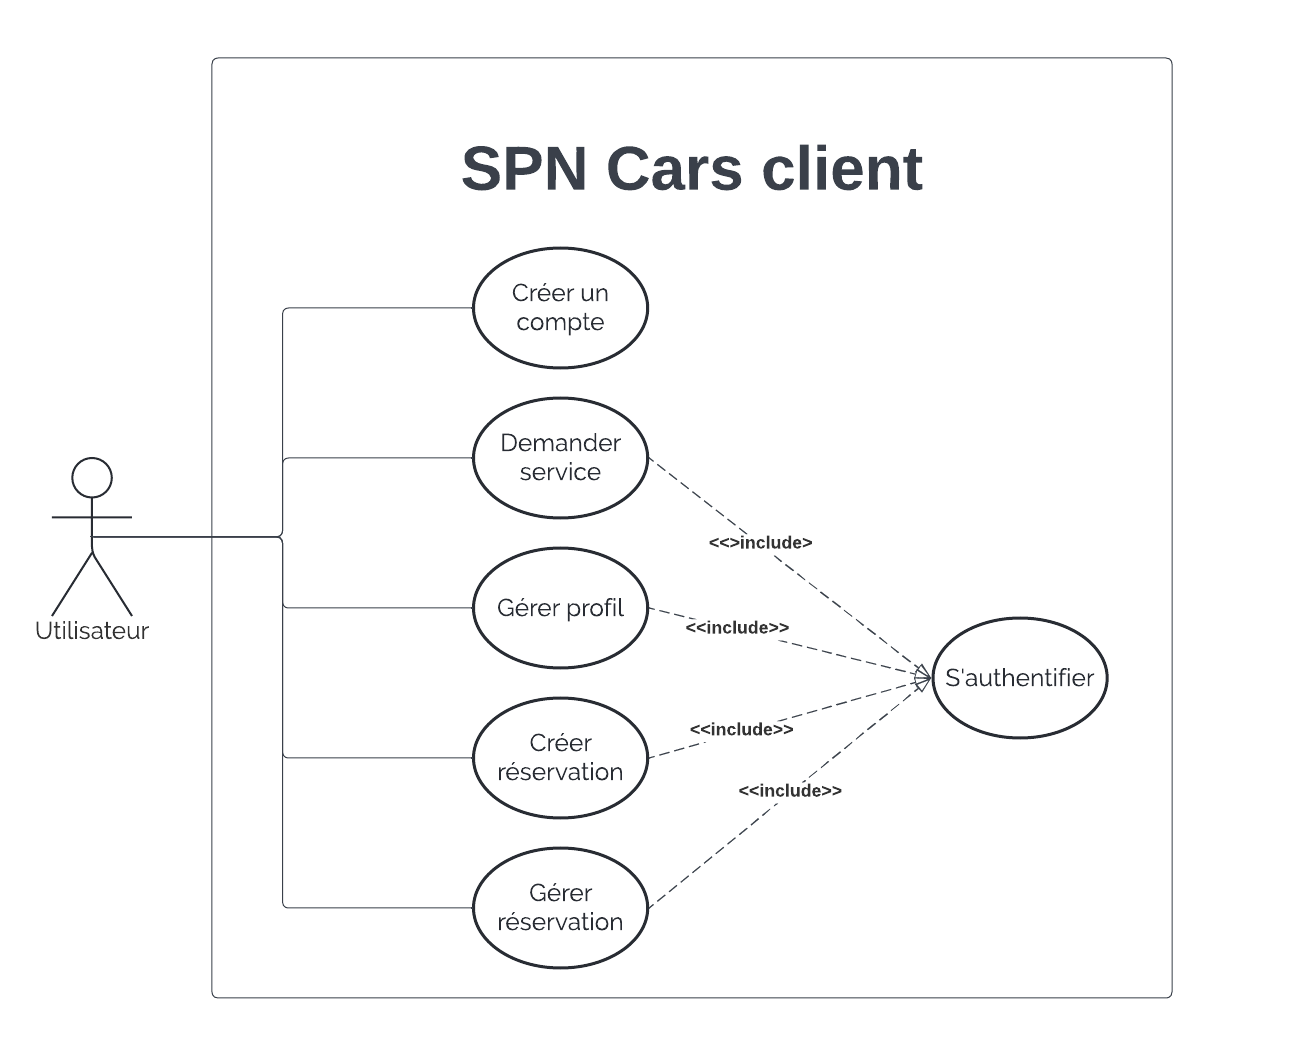
\includegraphics[height=0.5\textheight]{uml/use_cases.png}
    \vspace{1cm}
    \captionsetup{justification=centering}
    \caption{Diagramme de cas d'utilisation généralisé}
    \label{fig:use_case_diag}
\end{figure}
\subsubsection{Gérer profil}
L'utilisateur peut gérer son profil : Il peut changer sa photo de profil et ses informations personnels.\\
\begin{figure}[H]
    \centering
    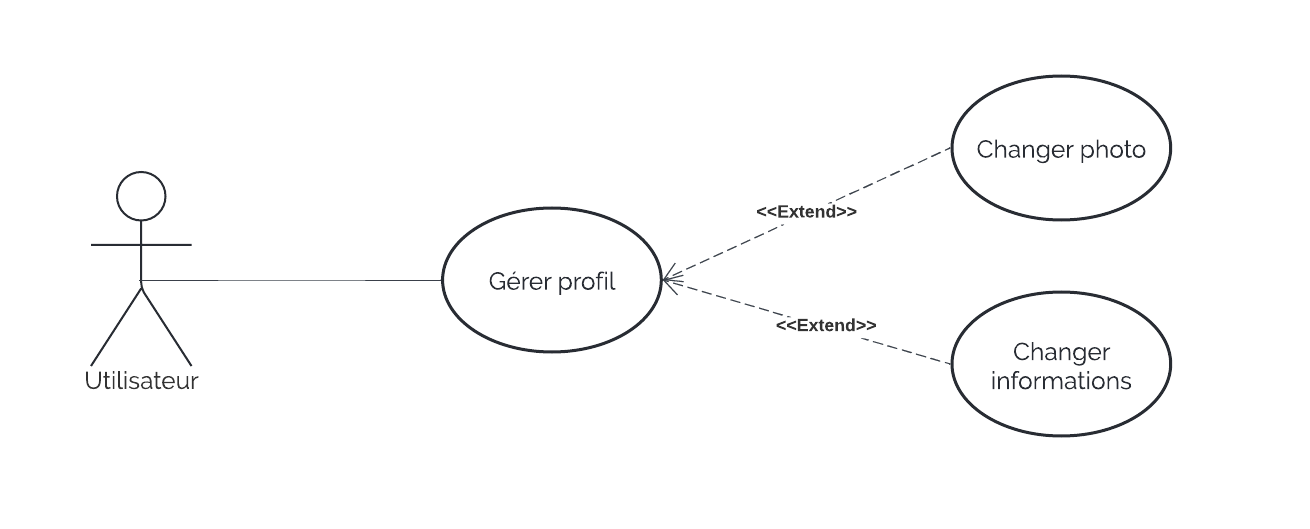
\includegraphics[width=\textwidth]{uml/profile_use_case.png}
    \vspace{1cm}
    \captionsetup{justification=centering}
    \caption{Diagramme de cas d'utilisation spécifique: Gestion de profil.}
    \label{fig:use_case_manage_profile}
\end{figure}
\subsection{Créer réservation}
Pour créer sa réservation, l'utilisatuer doit Louer une voiture, effectuer un paiement et signer le contrat numérique de location.\\
\begin{figure}[H]
    \centering
    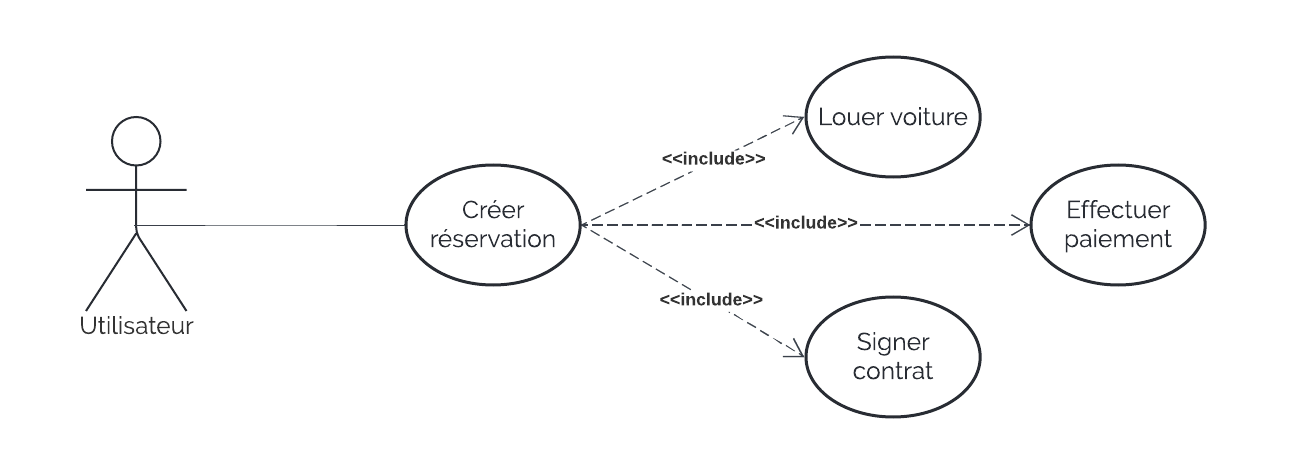
\includegraphics[width=\textwidth]{uml/reservation_use_case.png}
    \vspace{1cm}
    \captionsetup{justification=centering}
    \caption{Diagramme de cas d'utilisation spécifique: Créer réservation.}
    \label{fig:use_case_create_res}
\end{figure}
\subsection{Gérer réservation}
L'utilisateur peut gérer sa réservation, il peut suivre la position de la voiture louée en temps réel, et il peut aussi annuler sa réservation.
\begin{figure}[H]
    \centering
    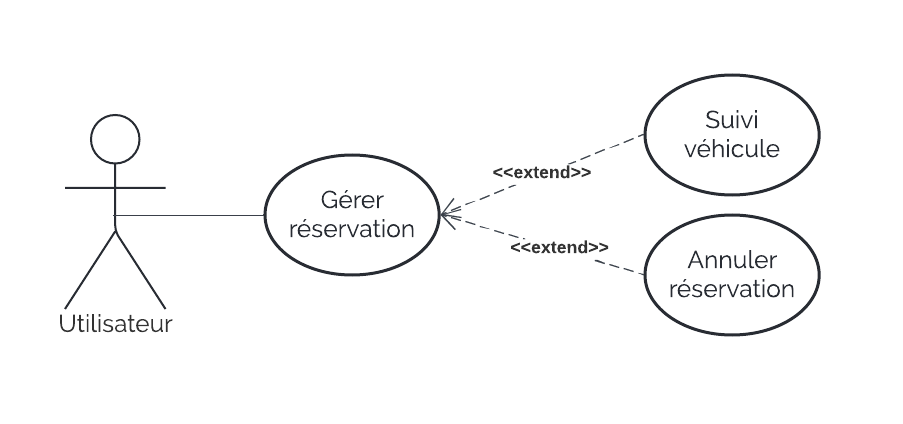
\includegraphics[width=\textwidth]{uml/manage_res_use_case.png}
    \vspace{1cm}
    \captionsetup{justification=centering}
    \caption{Diagramme de cas d'utilisation spécifique: Gérer réservation.}
    \label{fig:use_case_manage_res}
\end{figure}


\subsection{Diagramme de classes}
\begin{figure}[H]
    \centering
    \rotatebox[origin=c]{-90}{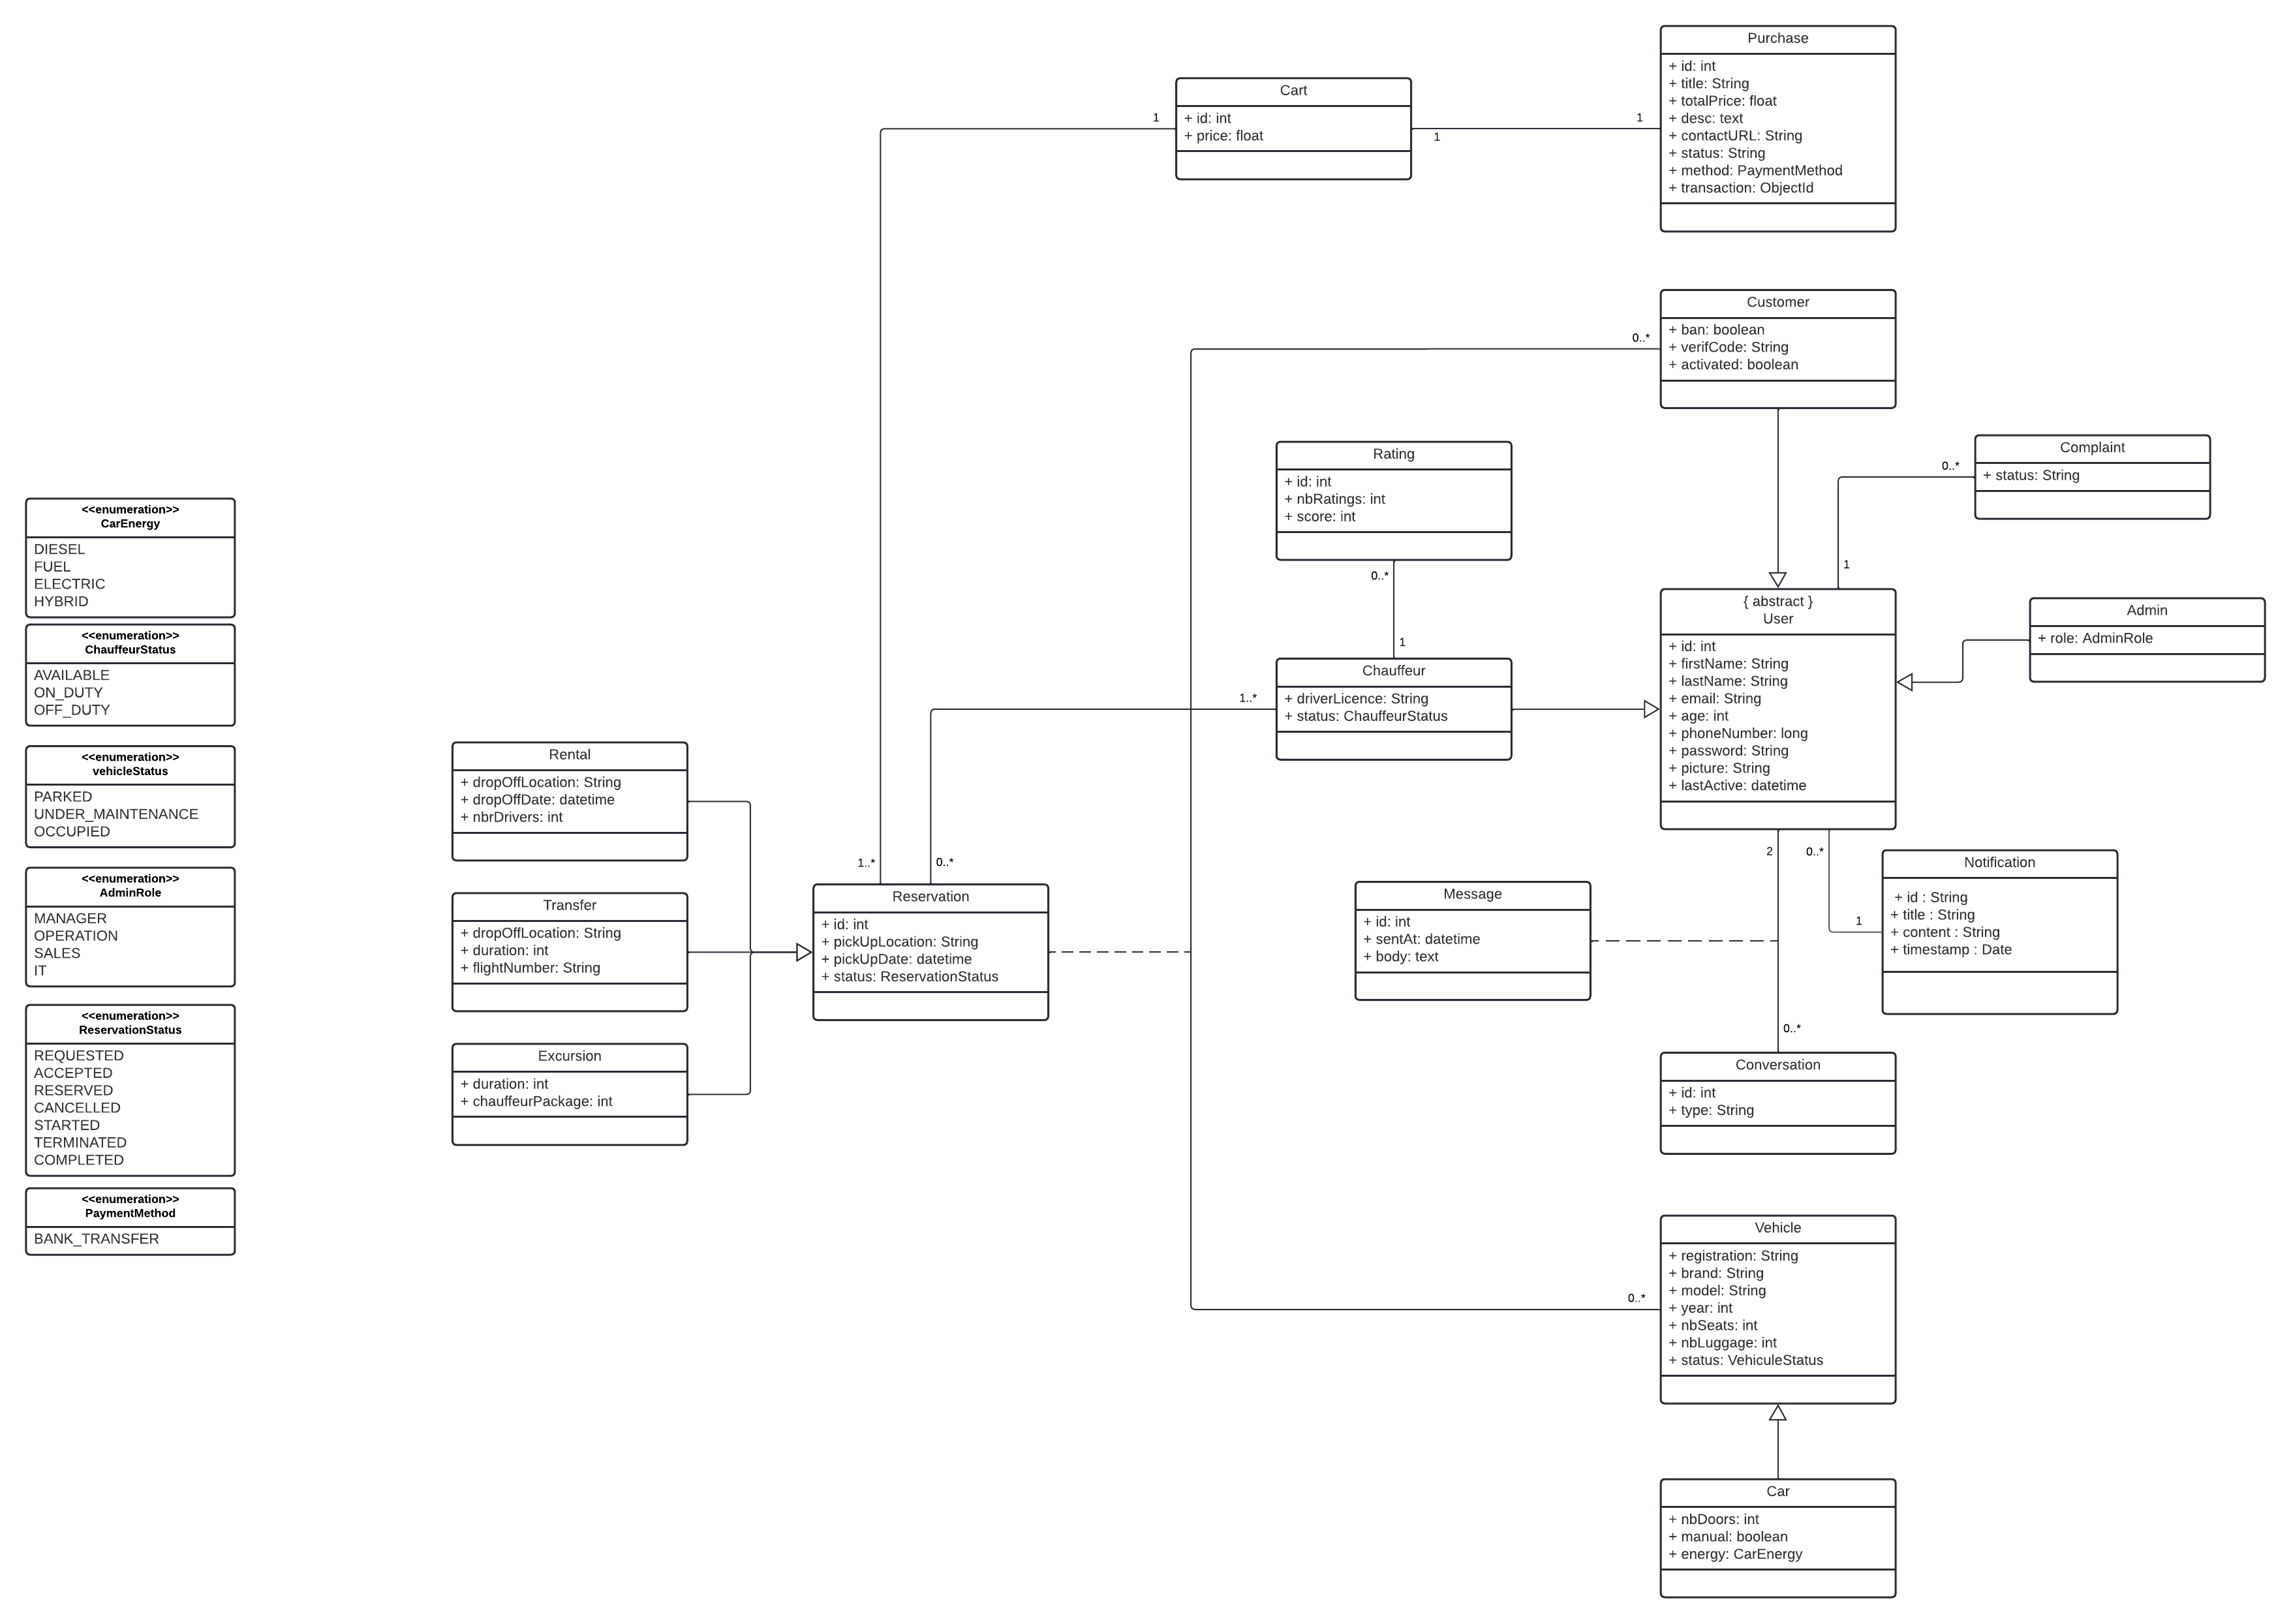
\includegraphics[width=0.9\textheight,height=\textwidth]{uml/class_diag.png}}
    \vspace{1cm}
    \captionsetup{justification=centering}

    \caption{Diagramme de classe}
    \label{fig:class_diag}
\end{figure}
\clearpage
\subsection{Diagrammes de séquences}
Les diagrammes de séquences sont le moyen qui permettent de décrire d'une manière détaillée les différents cas d'utilisation
\subsubsection{Création de compte}
\begin{figure}[H]
    \centering
    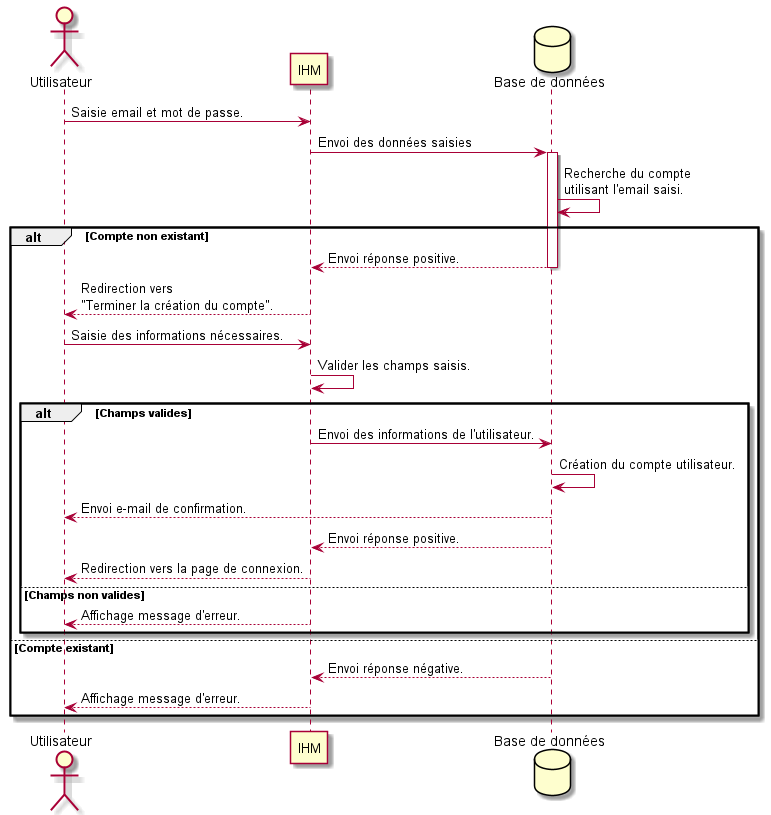
\includegraphics[width = \textwidth]{uml/register_email.png}
    \vspace{1cm}
    \captionsetup{justification=centering}

    \caption{Diagramme de séquence : Création de compte avec E-mail et mot de passe.}
    \label{fig:seq_register_email}
\end{figure}
\begin{figure}[H]
    \centering
    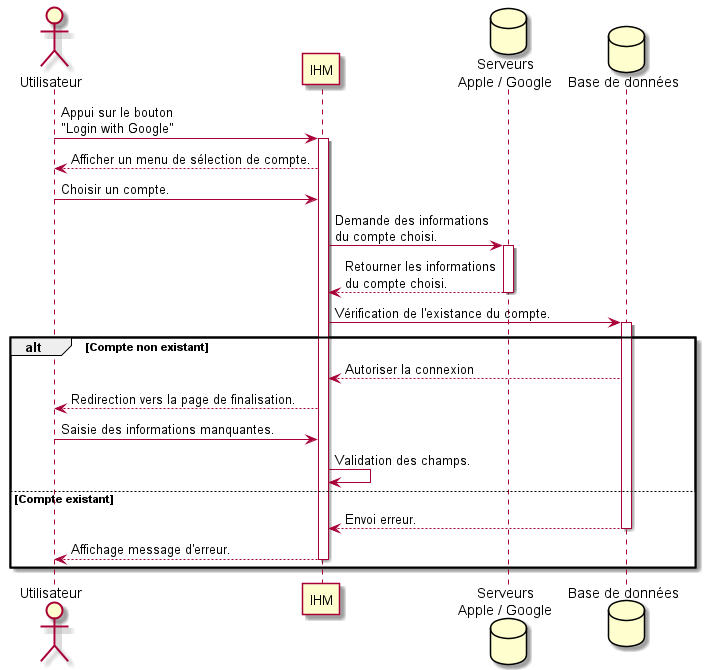
\includegraphics[width = \textwidth]{uml/apple_google.png}
    \vspace{1cm}
    \captionsetup{justification=centering}

    \caption{Diagramme de séquence : Création de compte avec Un compte Google / Apple.}
    \label{fig:seq_register_apple_google}
\end{figure}
\subsubsection{Authentification}
\begin{center}
    \begin{figure}[H]
        \centering
        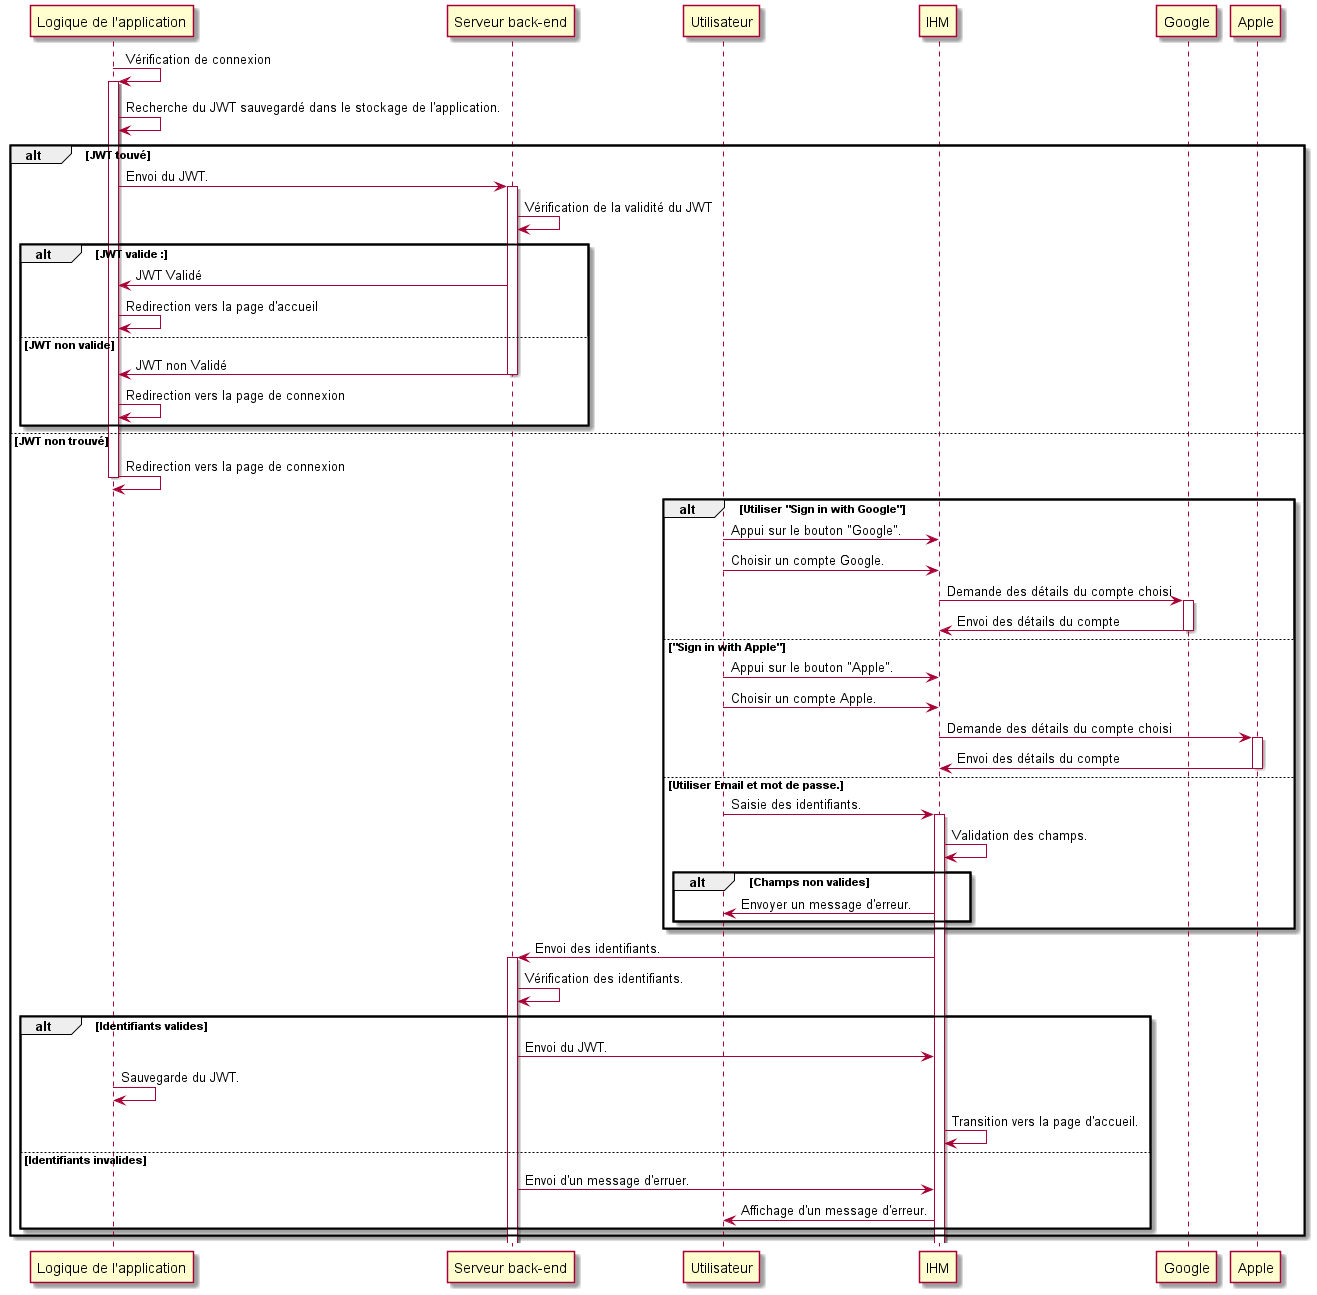
\includegraphics[width = \textwidth]{uml/Authentification.png}
        \vspace{1cm}
        \captionsetup{justification=centering}

        \caption{Diagramme de séquences: Authentification.}
        \label{fig:seq_auth}
    \end{figure}
\end{center}
\subsubsection{Page d'accueil}
\begin{figure}[H]
    \centering
    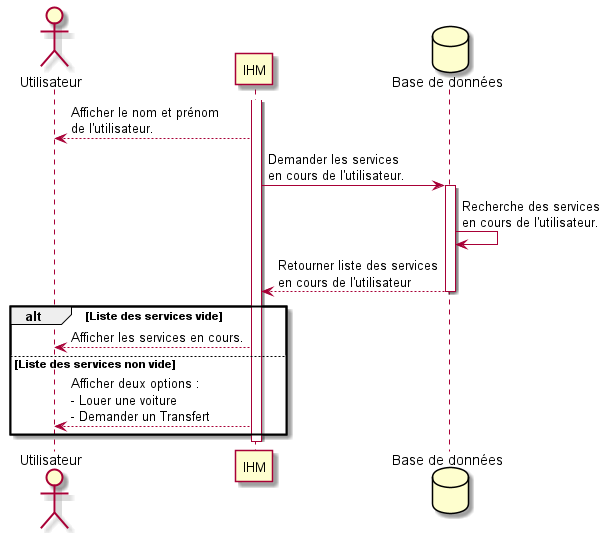
\includegraphics[width=\textwidth]{uml/home.png}
    \vspace{1cm}
    \caption{Diagramme de séquences : Page d'accueil.}
    \label{fig:seq_home}
\end{figure}
% \subsubsection{Gestion de profil}
\subsubsection{Demander un service}
\begin{figure}[H]
    \centering
    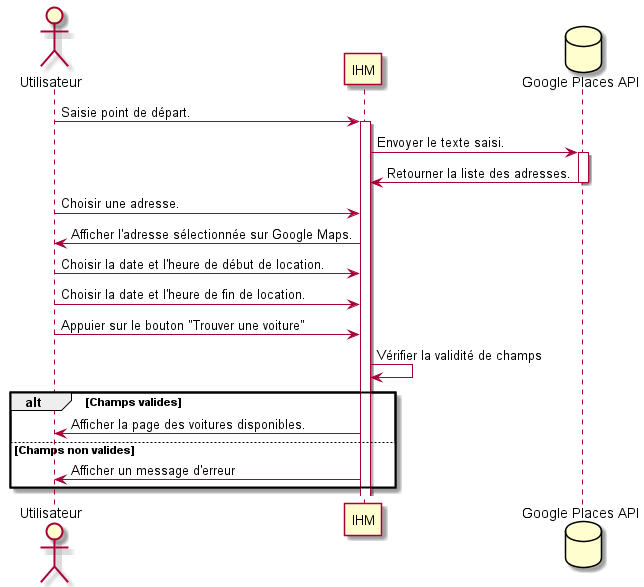
\includegraphics[width = \textwidth]{uml/rent a car.png}
    \vspace{1cm}
    \captionsetup{justification=centering}

    \caption{Diagramme de séquences: Demander une location.}
    \label{fig:seq_location}
\end{figure}
\vspace{1cm}
\begin{figure}[H]
    \centering
    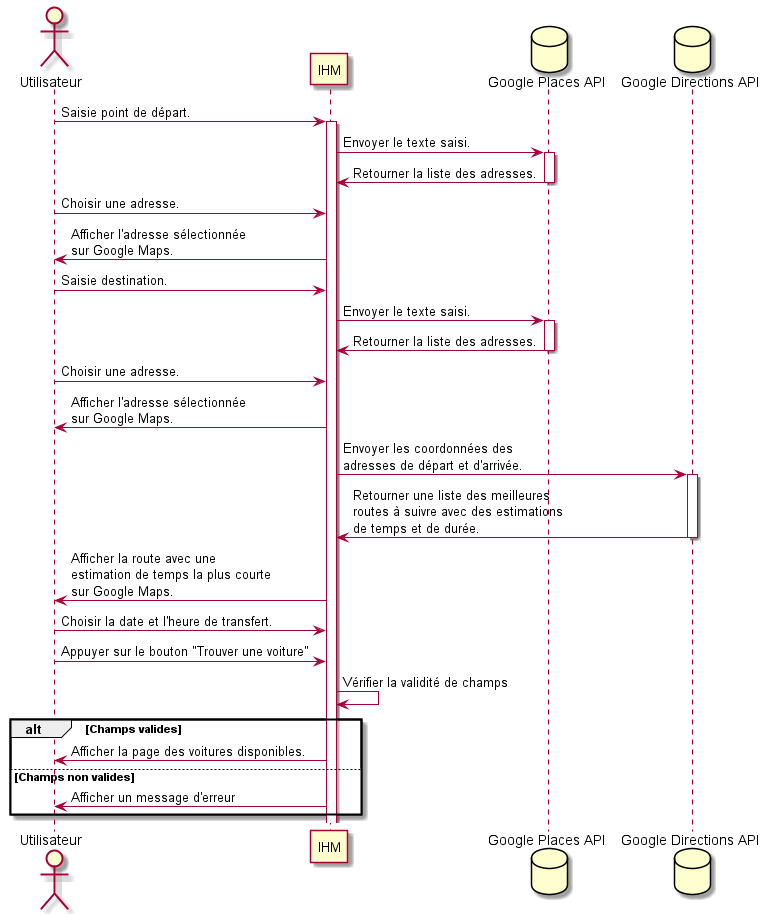
\includegraphics[width = \textwidth]{uml/transfert.png}
    \vspace{1cm}
    \captionsetup{justification=centering}

    \caption{Diagramme de séquences: Demander un transfert.}
    \label{fig:seq_transfert}
\end{figure}
\subsubsection{Affichage des voitures disponibles}
\begin{figure}[H]
    \centering
    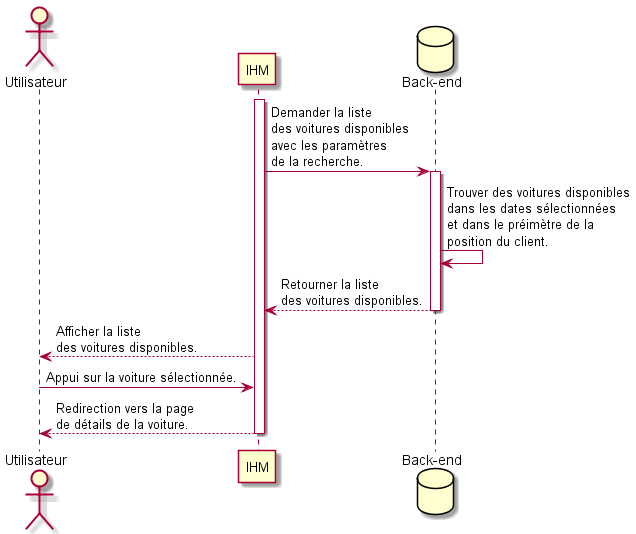
\includegraphics[width = \textwidth]{uml/choisir voiture.png}
    \vspace{1cm}
    \captionsetup{justification=centering}

    \caption{Diagramme de séquences : Choisir une voiture}
    \label{fig:seq_car_select}
\end{figure}
\subsubsection{Signature numérique de contrat de location}
\begin{figure}[H]
    \centering
    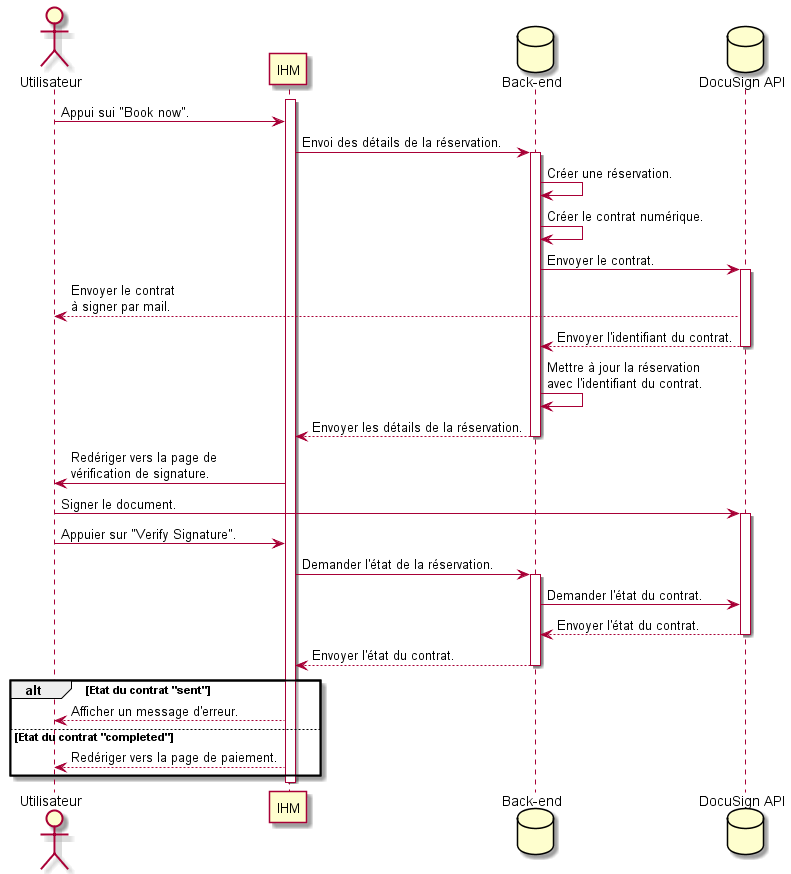
\includegraphics[width = \textwidth]{uml/docusign.png}
    \captionsetup{justification=centering}
    \caption{Diagramme de séquences : Envoi du contrat de location.}
    \label{fig:seq_location_contract}
\end{figure}
\subsubsection{Paiement en ligne}
\begin{figure}[H]
    \centering
    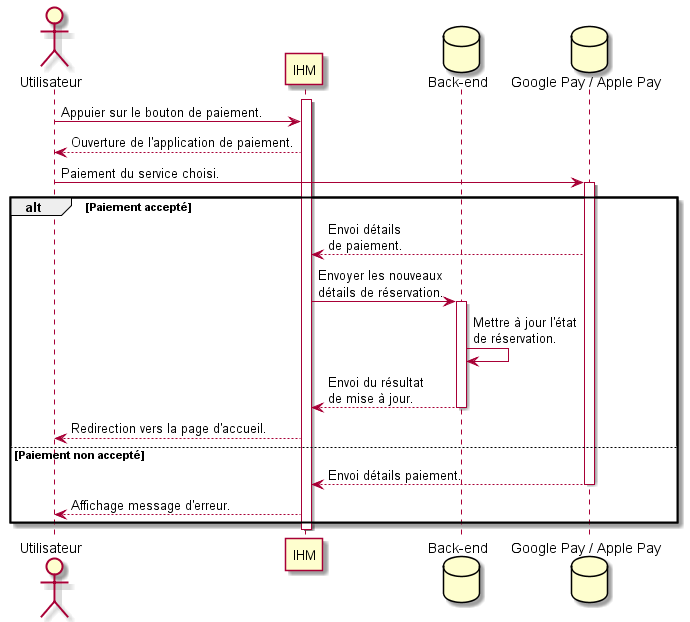
\includegraphics[width = \textwidth]{uml/payment.png}
    \captionsetup{justification=centering}
    \caption{Diagramme de séquences: Paiement des services.}
    \label{fig:seq_payment}
\end{figure}
\subsubsection{Localiser une voiture}
\section{UI/UX Design}
Avant de passer au développement de l'application, il faut créer d'abord les prototypes des interfaces utilisateur. \\
\noindent Cette étape est nécessaire pour tester plusieurs approches dans les interfaces de l'application, s'assurer d'offrir une expérience optimale pour l'utilisateur. \\
\noindent Suite à une collaboration avec l'équipe de design UI/UX, les interfaces suivantes ont été créées.
\vspace{1cm}
\begin{multicols}{2}
    \begin{figure}[H]
        \centering
        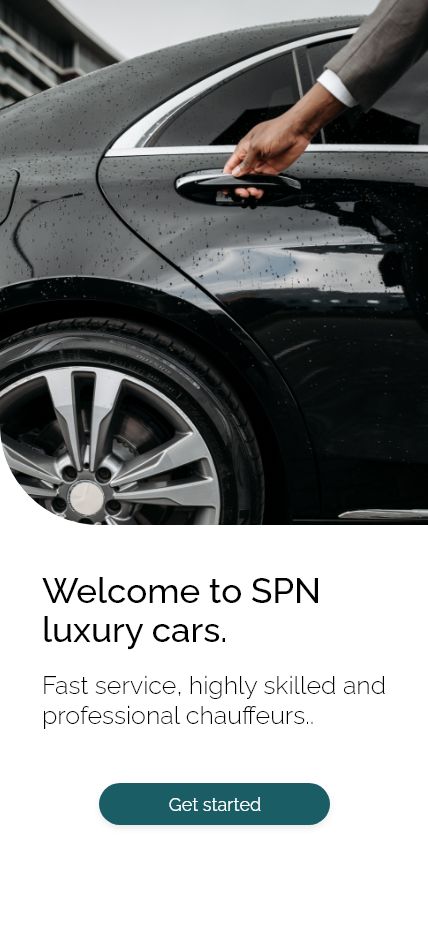
\includegraphics[width=0.25\textwidth]{ui_screenshots/Guide.png}
        \vspace{1cm}
        \captionsetup{justification=centering}

        \caption{Première page.}
        \label{fig:start_page}
    \end{figure}
    \begin{figure}[H]
        \centering
        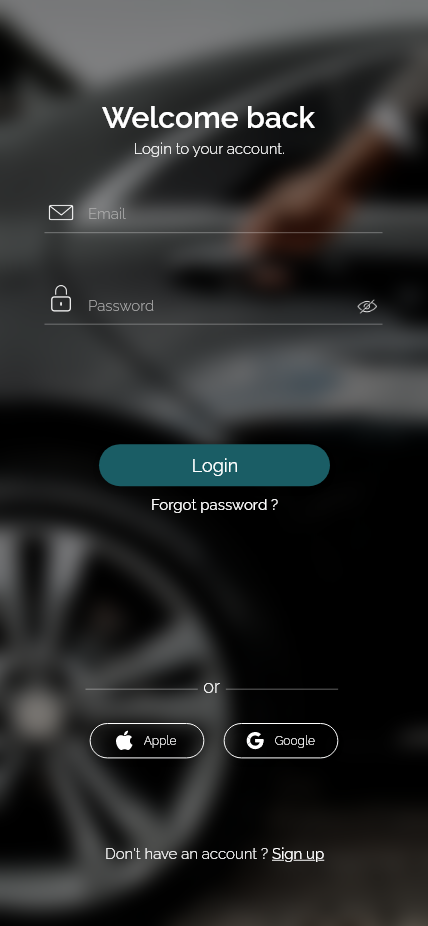
\includegraphics[width=0.25\textwidth]{ui_screenshots/sign in.png}
        \vspace{1cm}
        \captionsetup{justification=centering}

        \caption{Page de connexion.}
        \label{fig:sign_in_page}
    \end{figure}
\end{multicols}
% \newpage
\begin{multicols}{2}
    \begin{figure}[H]
        \centering
        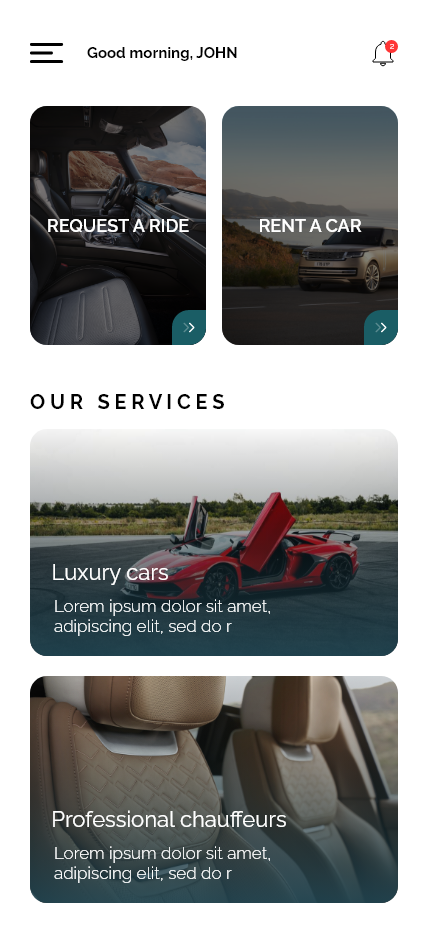
\includegraphics[width=0.25\textwidth]{ui_screenshots/No Active trip.png}
        \vspace{1cm}
        \captionsetup{justification=centering}

        \caption{\centering Page d'accueil.}
        \label{fig:no_active_trip}
    \end{figure}
    \begin{figure}[H]
        \centering
        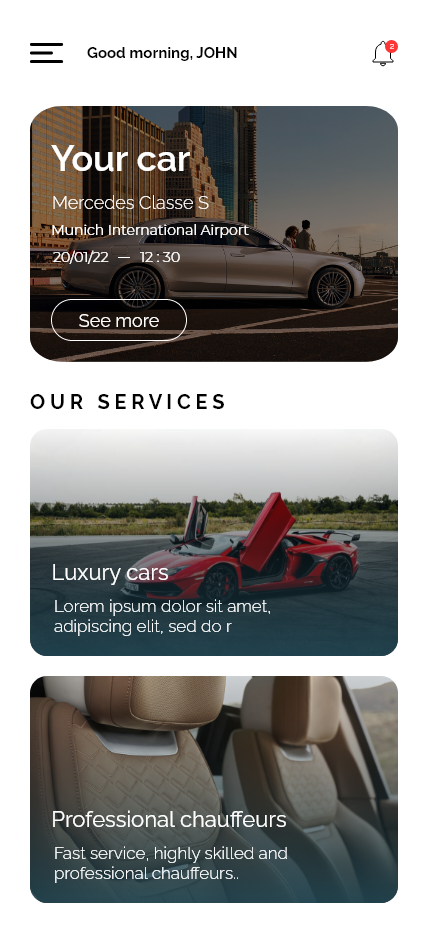
\includegraphics[width=0.25\textwidth]{ui_screenshots/Active trip.png}
        \vspace{1cm}
        \captionsetup{justification=centering}

        \caption{\centering Page d'accueil lors d'un transfert en cours.}
        \label{fig:active_trip}
    \end{figure}
\end{multicols}
\clearpage
\begin{multicols}{2}
    \begin{figure}[H]
        \centering
        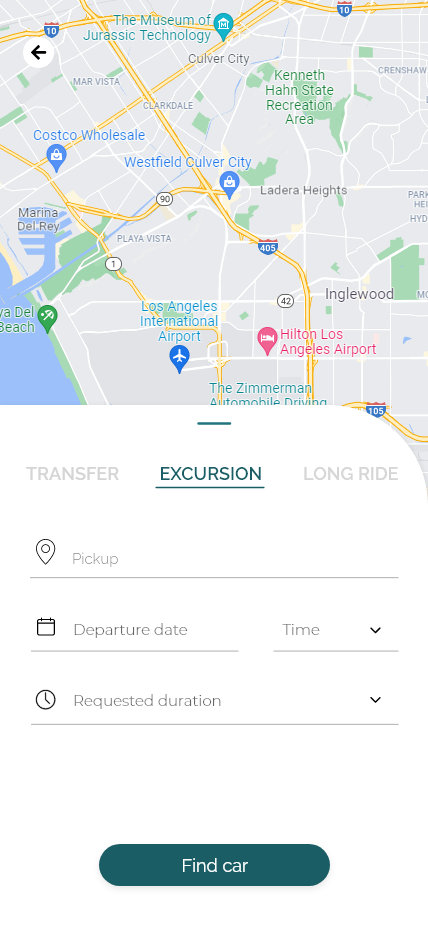
\includegraphics[width=0.25\textwidth]{ui_screenshots/Excursion.png}
        \vspace{1cm}
        \captionsetup{justification=centering}

        \caption{\centering Sélection de type de transfert.}
        \label{fig:trip_select}
    \end{figure}
    \begin{figure}[H]
        \centering
        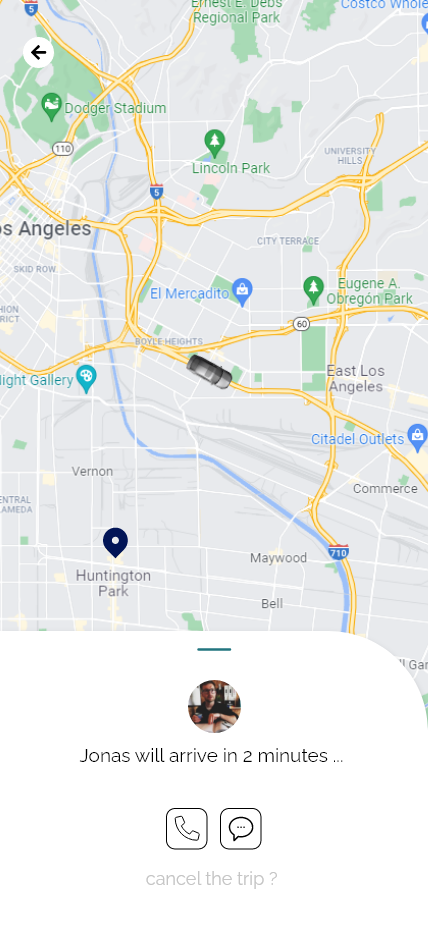
\includegraphics[width=0.25\textwidth]{ui_screenshots/Map view.png}
        \vspace{1cm}
        \captionsetup{justification=centering}

        \caption{\centering Suivi de la position actuelle du chauffeur avec la voiture.}
        \label{fig:follow_driver}
    \end{figure}
\end{multicols}
\begin{multicols}{2}
    \begin{figure}[H]
        \centering
        \includegraphics[width=0.25\textwidth]{ui_screenshots/Available cars – 1.png}
        \vspace{1cm}
        \captionsetup{justification=centering}

        \caption{\centering Liste de voitures disponibles.}
        \label{fig:available_cars}
    \end{figure}
    \begin{figure}[H]
        \centering
        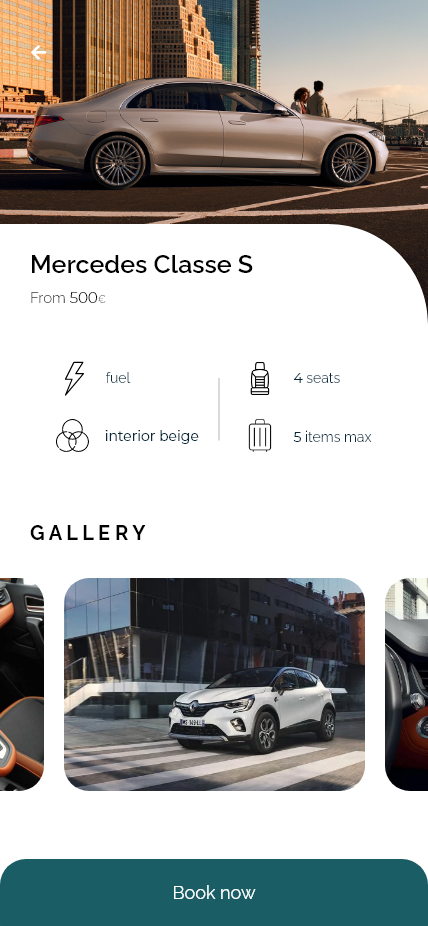
\includegraphics[width=0.25\textwidth]{ui_screenshots/Car details.png}
        \vspace{1cm}
        \captionsetup{justification=centering}

        \caption{\centering Détails de la voiture sélectionnée.}
        \label{fig:car_details}
    \end{figure}
\end{multicols}
\vspace{1cm}
\begin{figure}[H]
    \centering
    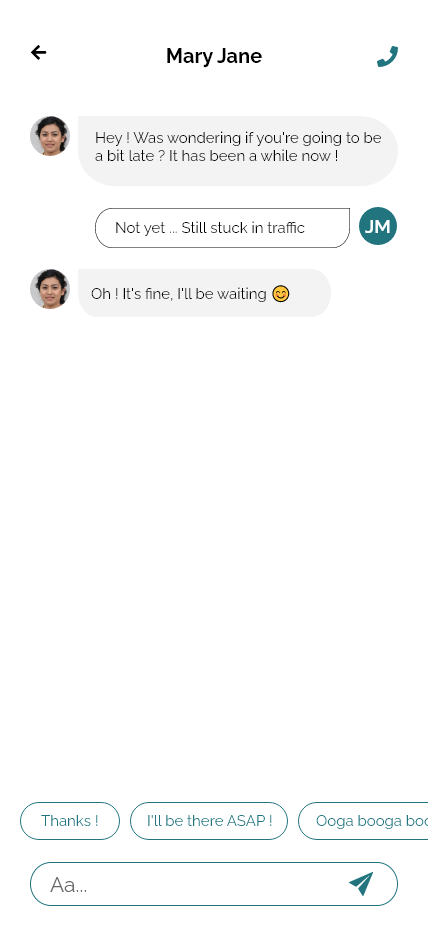
\includegraphics[width=0.25\textwidth]{ui_screenshots/DMs.png}
    \vspace{1cm}
    \caption{\centering Messagerie instantannée avec le chauffeur.}
    \label{fig:dms}
\end{figure}
\section{Technologies et outils utilisés}
Comme cette application sera une application mobile, il est nécessaire que la performance soit la priorité lors du développement. C'est pourquoi on a choisi les technologies suivantes pour offrir une application rapide, performante, facile à utiliser.\\
\noindent Ses différentes technologies sont classifiés dans trois domaines principalement : Conception des interfaces graphiques, développement de l'application, et développement du back-end de l'application.\\
\subsection{Flutter}
\vspace{1cm}
\begin{figure}[H]
    \centering
    
\includegraphics[width=0.25\textwidth]{flutter.png}
    \vspace{1cm}
    \captionsetup{justification=centering}

    \caption{Logo Flutter}
    \label{fig:flutter_logo}
\end{figure}
\textit{\textbf{Flutter}} \cite{flutter} est un kit de développement (SDK) open-source créé par Google et publié en 2017.\\
\noindent Flutter permet de créer des application mobiles (Android / iOS), web et meême desktop (Windows / Linux / MacOS), avec une seule base de code en Dart, un langage de programmation développé aussi par Google. \\
\noindent Flutter présente plusieurs avantages qui permettent de créer des applications mobiles performantes et réduit aussi le coût et le temps de développement nécessaires, grâce au langage de programmation utilisé \textit{\textbf{Dart}} qui est très facile à maîtriser et qui offre plusieurs avantages, dont le plus important la fonctionnalité de <<\textit{\textbf{Hot Reload}}>> qui permet de recharger l'application et afficher les changements sur l'écran sans passer par la recompilation du code source.
\subsection{Express JS}
\vspace{1cm}
\begin{figure}[H]
    \centering
    
\includegraphics[width=0.25\textwidth]{express.png}
    \vspace{1cm}
    \captionsetup{justification=centering}
    \caption{Logo Express}
    \label{fig:express_logo}
\end{figure}
\textit{\textbf{Express JS}} \cite{expressjs} est un framework back-end gratuit et open-source pour NodeJS. Créé par TJ Holowaychuk, la première version publique d'Express JS a été introduite au public en 2010.\\
Express JS est un framework minimaliste, très léger pour garantir une performance optimale et une exécution rapide. Ce framework est aussi très flexible, même s'il fournit que quelques fonctionnalités, grâce à \textit{\textbf{NPM}}, le gestionnaire de packets de NodeJS, il peut être complété par plusieurs librairies disponibles.\\
\noindent Grâce à son minimalisme et facilité d'implémentation, ExpressJS est utilisé par plusieurs par nombreuses sociétés dans le monde, pour développer tout type d'applications, parmi ses sociétés il y a des géants de technologies tels que \textit{\textbf{IBM}}, \textit{\textbf{Uber}}, et plusieurs autres.
\subsection{JSON Web Token (JWT)}
\begin{figure}[H]
    \centering
    
\includegraphics[width=0.25\textwidth]{jwt.png}
    \vspace{1cm}
    \captionsetup{justification=centering}
    \caption{Logo JWT}
    \label{fig:jwt_logo}
\end{figure}
\textbf{\textit{Josn Web Token}} ou tout simplement connu comme "JWT" est un standard créé en 2015, qui permet d'encapsuler des données dans des jetons et l'échanger entre plusieurs parties en toute ssécurité.

Un jeton est compsé principalement de trois parties :
\begin{itemize}
    \item Un en-tête qui décrit le jeton en format JSON.
    \item Le contenu de ce jeton qui est également en format JSON.
    \item Une signature numérique.
\end{itemize}
\subsection{MongoDB}
\vspace{1cm}
\begin{figure}[H]
    \centering
    
\includegraphics[width=0.25\textwidth]{mongo.png}
    \vspace{1cm}
    \captionsetup{justification=centering}

    \caption{Logo MongoDB}
    \label{fig:mongo_logo}
\end{figure}
\textit{\textbf{MongoDB}} \cite{mongodb} , est un système de gestion de base de données NoSQL, orientée documents. Une base de données NoSQL est utilisée pour le stockage de volumes massifs de données, elle se distingue des des bases de données relationnelles par sa flexibilité et ses performances.\\
\noindent Le système MongoDB est développé par la société qui porte le même nom en 2007. Cette entreprise travaillait sur un système de cloud computing à données largement réparties.\\
\noindent Il est depuis devenu l'un des systèmes de gestion de base de données les plus utilisées, notamment pour des sites web très populaires tels que : \textit{\textbf{SourseForge.net}}, \textit{\textbf{eBay}} et \textit{\textbf{The New York Times}}.\\
\noindent Contrairement à une base de données relationnelle SQL traditionnelle, MongoDB ne repose pas sur des tableaux et des colonnes. Les données sont stockées sous forme de collections et de documents.
Les documents sont des paires de valeurs / clés servant d'unité de données de base. Les collections quant à elles contiennent des ensembles de documents et de fonctions. Elles sont l'équivalent des tableaux dans les bases de données relationnelles classiques.
\subsection{Firebase}
\vspace{1cm}
\begin{figure}[H]
    \centering
    
\includegraphics[width=0.25\textwidth]{firebase.png}
    \vspace{1cm}
    \captionsetup{justification=centering}

    \caption{Logo Firebase}
    \label{fig:firebase_logo}
\end{figure}
\textit{\textbf{Firebase}} \cite{firebase} est une plateforme créée en 2011, puis acquise et développée par Google en 2014. Firebase facilite la création de back-end à la fois scalable et performant.\\
\noindent L'objectif de firebase est d'offrir aux professionnels et aux particuliers un moyen d'éviter l'engagement dans un processus complexe de création et de maintenance d'une architecture serveur.\\
\noindent Firebase offre des API intuitives regroupées dans un SDK unique. Ces API permettent de gagner du temps et de réduire le nombre d'intégrations qu'on doit gérer dans l'application.\\
\noindent Firebase offre plusieurs services que tout le monde peut utiliser gratuitement grâce à sa politique <<pay as you go>> qui nécessite le paiement de ses services seulement si l'utilisation des ressources dépasse le quota du plan gratuit offert. Les services de Firebase les plus utilisés sont :
\begin{itemize}
    \item \textbf{Firestore}:\\ Une base de données NoSQL, bénéficiant d'un hébergement cloud et permettant le stockage et la synchronisation de données des untilisateurs.
    \item \textbf{Fireabse Authentification}:\\ Un SDK prêt et facile à exploiter qui permet de d'authentifier les utilisateurs en offrant plusieurs méthodes d'authentification tels que Google, Apple, Facebook, Email et mot de passe, numéro de téléphone et plusieurs d'autres méthodes pour assurer l'authentification de l'utilisateur.
    \item \textbf{Firebase Cloud Messaging}:\\ Permet de connecter plusieurs périphériques au serveur dans les meilleures conditions (fiabilité et économie de batterie). Ce service permet de recevoir et envoyer des notification sur les différentes plateformes (Web / iOS / Android). Avec Firebase Cloud Messaging, il est possible aussi d'assurer un service de messagerie instantanée entre les utilisateurs.
\end{itemize}
\begin{figure}[H]
    \centering
    
\includegraphics[width=0.25\textwidth]{git.png}
    \vspace{1cm}
    \captionsetup{justification=centering}
    \caption{Logo Git}
    \label{fig:git_logo}
\end{figure}
\subsection{Visual Studio Code}
\textit{\textbf{Visual Studio Code}} \cite{vscode} est un éditeur de texte open-source développé par Microsoft \cite{microsoft} pour Windows MacOS et Linux en 2015. Riche en fonctionnalités tels que le support de déboguage, complétion intelligente du code, intégration de système de contrôle de version Git,et la capabilité d'installation d'extentions qui permettent d'améliorer l'expérience de l'utilisateur, Visual Studio Code est devenu l'un des premier choix pour plusieurs developpeurs pour travailler sur leurs différents projets.
\subsection{Postman}
\begin{figure}[H]
    \centering
    
\includegraphics[width=0.25\textwidth]{postman.png}
    \vspace{1cm}
    \captionsetup{justification=centering}
    \caption{Logo Postman.}
    \label{fig:postman_logo}
\end{figure}
\textit{\textbf{Postman}} \cite{postman} est une plateforme permettant de concevoir, développer, et tester des API. Crée en 2012 comme une extension pour Google Chrome, Postman a gagné une grande popularité, qui l'a permis de migrer vers une application pour Windows MacOS, et Linux. Postman maintenant est le premier choix pour la plupart des développeurs, avec plus de 20 millions d'utilisateurs \cite{postman_users}.
\subsection{Adobe Xd}
\vspace{1cm}
\begin{figure}[H]
    \centering
    
\includegraphics[width=0.25\textwidth]{xd_logo.png}
    \vspace{1cm}
    \captionsetup{justification=centering}

    \caption{Logo Adobe Xd}
    \label{fig:xd_logo}
\end{figure}
\textit{\textbf{Adobe Xd}} \cite{adobe_xd} est un outil de conception et modélisation des interfaces utilisateur des applications web et mobiles, développé par Adobe Inc.\\
\noindent Grâce aux outils fournis par Adobe Xd, la conception, l'amélioration et la rectification des interfaces graphiques et l'expérience de l'utilisateur de l'application sera plus facile, plus rapide et plus efficace.
\noindent Dans le cadre de ce projet, Adobe Xd a été utilisé pour la création des prototypes des interfaces graphiques, qui seront, par la suite, construits en application mobile à l'aide de Flutter.
\subsection{Git}
\vspace{1cm}
\begin{figure}[H]
    \centering
    
\includegraphics[width=0.25\textwidth]{vscode.png}
    \vspace{1cm}
    \captionsetup{justification=centering}

    \caption{Logo Visual Studio Code.}
    \label{fig:vscode_logo}
\end{figure}
\textit{\textbf{Git}} \cite{git} est un système de contrôle de version open-source créé en 2005 par \textit{\textbf{Linus Torvalds}}, le créateur du noyau du système d'exploitation Linux.\\
\noindent Git permet de gérer les ajouts et changements apportés au code source de manière tracée. Ainsi, si une erreur est commise, les développeurs peuvent revenir en arrière et comparer les versions antérieures du code, ce qui leur permet de corriger l'erreur tout en minimisant les perturbations pour tous les membres de l'équipe.
\subsection{Swagger}
\vspace{1cm}
\begin{figure}[H]
    \centering
    
\includegraphics[width=0.25\textwidth]{swagger.png}
    \vspace{1cm}
    \captionsetup{justification=centering}

    \caption{Logo Swagger}
    \label{fig:swagger_logo}
\end{figure}
\textit{\textbf{Swagger}} \cite{swagger} est un langage permettant de créer une description des API Restful à l'aide de JSON. A l'aide de ses outils Open-Source, Swagger permet de concevoir, créer et décrire des API REST.\\
\noindent Swagger est créer en 2011 par Tony Tam, cofondateur du site de dictionnaires Wordnik, suite à un besoin d'automatisation de documentation de l'API qui est devenue de plus en plus frustrante. Juste après sa création, le projet Swagger est devenu open-source en septembre 2011.\\
\noindent Swagger est maintenant maintenu par la société \textit{\textbf{SmartBear Software}} qui, en novembre 2015, de créer une organisation appelée \textit{\textbf{OpenAPI initiative}} dont diverses entreprises tels que Google, IBM et Microsoft sont les membres fondateurs.\\
\section*{Conclusion}
A travers ce chapitre, on a établi la conception de l'application SPN-Cars: On a dégager les besoins fonctionnels et non fonctionnels, qui, à travers eux on a pu créer les diagrammes de cas d'utilisation, les diagrammes de classes, et les diagrammes de séquences. Suite au développement de ces diagrammes, on a passé vers l'étape de conception des interfaces utilisateur. Toutes ces différentes étapes ont permit de choisir les technologies et outils qui seront utilisés pour la création de cette application.\\
Une fois les différents aspects de l'applications sont bien définis, on passera vers la phase de réalisation où on appliquera les diagrammes et interfaces développés dans ce chapitre pour produire cette application.
% Réalisation de l'application
\newpage
\chapter{Réalisation de l'application}
\minitoc
\clearpage
\section{Introduction} Dans ce chapitre, on décrira toutes les fonctionnalités de l'application, leurs fonctionnement, les différents scénarii d'exécution avec des captures d'écran de chaque interface d'utilisateur avec un diagramme de séquences qui décrit en détail la fonctionnalité mentionnée
\justifying
\section{Création de compte}
La première étape pour utiliser l'application SPN-Cars est de créer un compte. Ce compte permettra aux utilisateurs de bénéficier de tous les services offerts par l'application.\\
\noindent Pour créer un compte, l'utilisateur a la possibilité de choisir trois méthodes : Créer un compte avec son émail et choisir un mot de passe, ou créer un compte tout simplement en utilisant l'option de création de compte avec son compte Google ou Apple.
\subsection{Création de compte avec email et mot de passe}
C'est la méthode la plus basique qui existe depuis toujours. Pour créer un compte, l'utilisateur doit tout d'abord entrer son adresse email, un mot de passe, et une confirmation de ce mot de passe. Lors de l'appui sur le bouton de <<Créer un compte>>, l'application envoie une requête vers le serveur back-end afin de vérifier l'existence d'un compte d'utilisateur utilisant la même adresse e-mail. Après une recherche effectuée sur les utilisateurs, le serveur back-end envoie une réponse positive s'il n'a trouvé aucun compte d'utilisateur utilisant l'adresse e-mail entrée par l'utilisateur, sinon une réponse négative sera envoyée. Selon la réponse retournée par le serveur l'application redirigera l'utilisateur vers une page pour compléter l'étape de création de compte si la réponse du serveur est positive, ou affiche un message d'erreur avec l'erreur adéquate si la réponse du serveur est négative.
\newpage
\begin{multicols}{2}
    \begin{figure}[H]
        \begin{center}
            \centering
            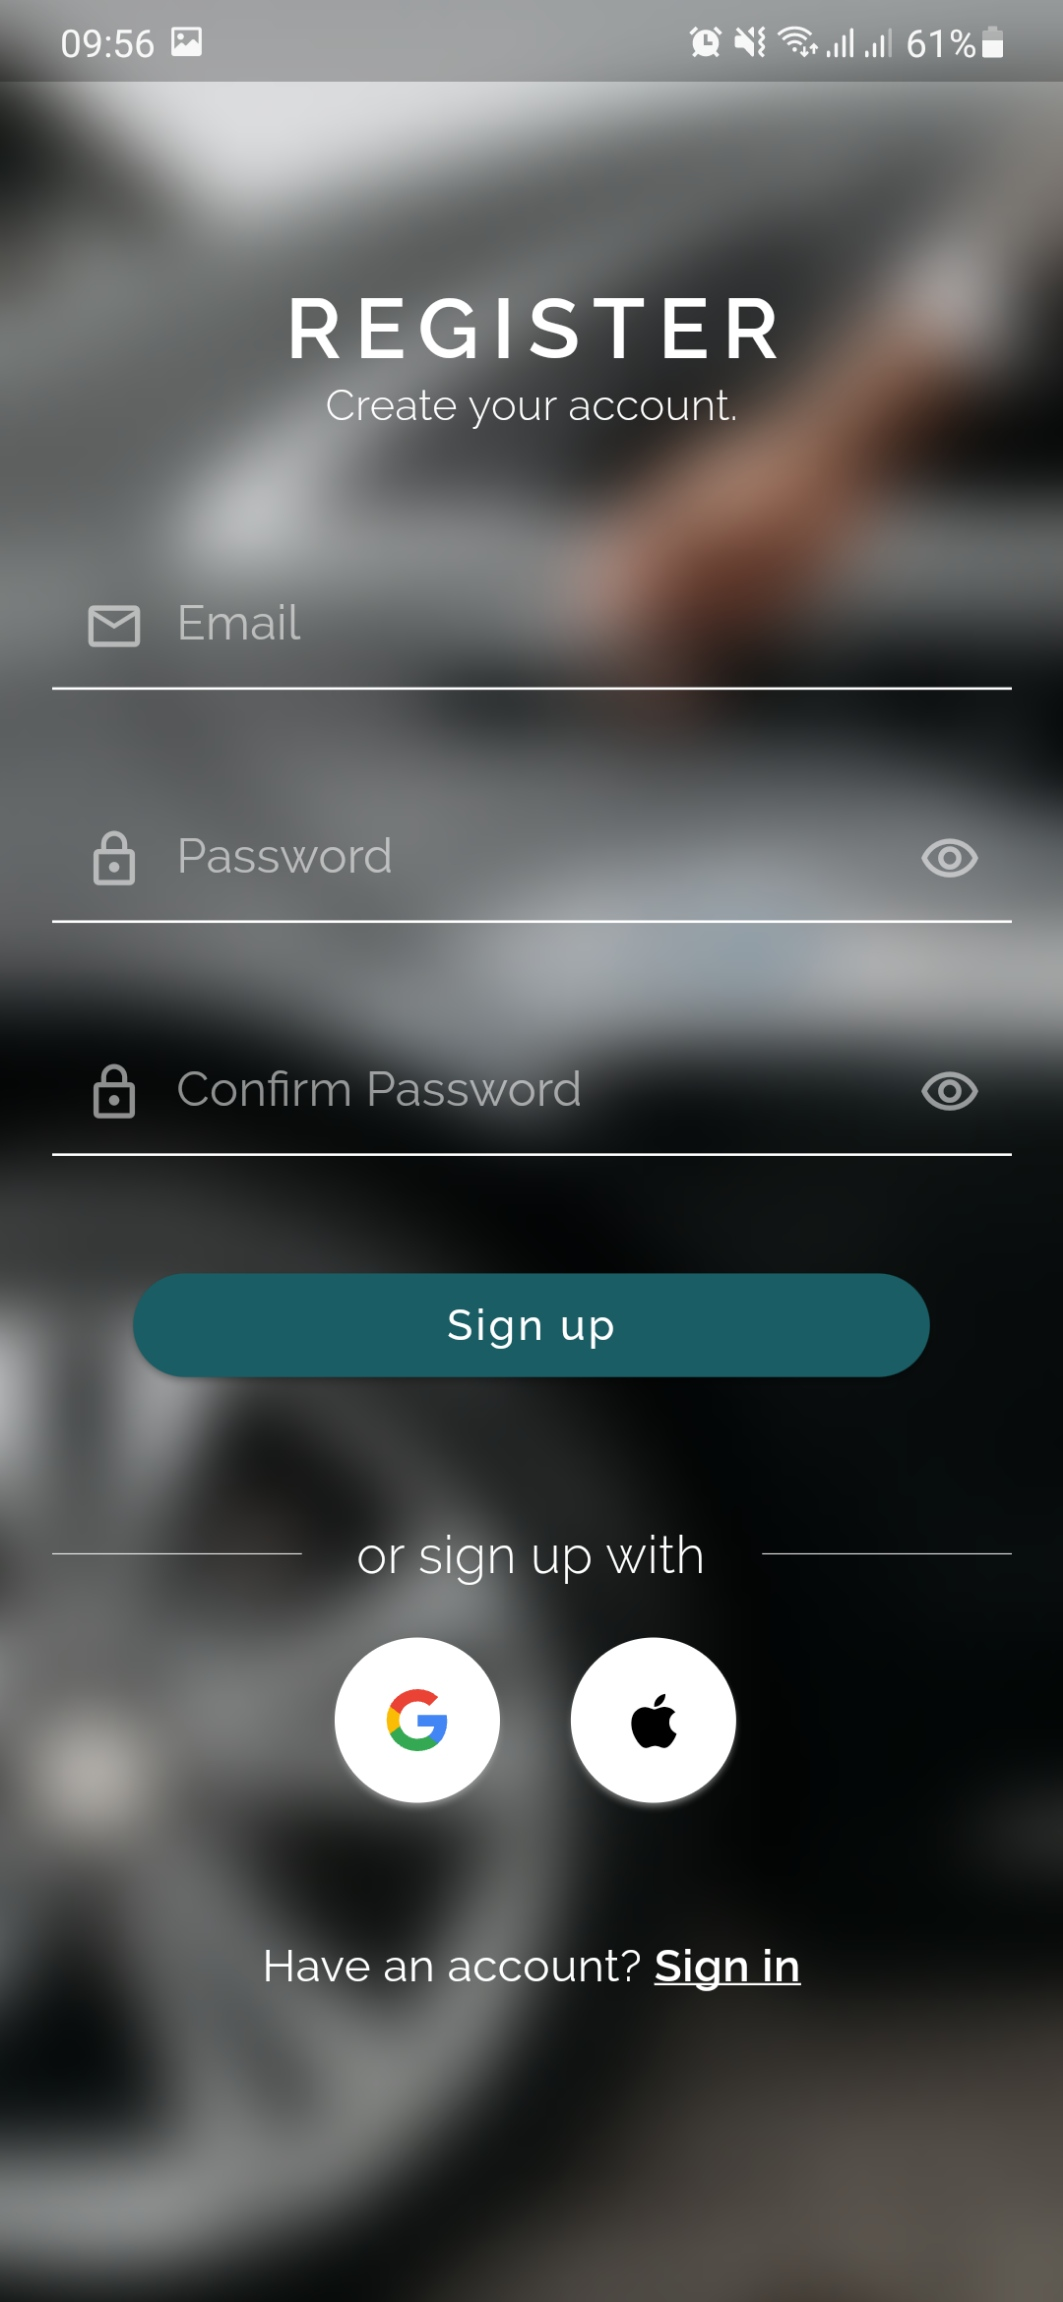
\includegraphics[height = 0.4 \textheight]{ui_screenshots/app_screenshots/register.png}
            \captionsetup{justification=centering}
            \caption{Formulaire de création de compte : 1ère étape.}
            \label{fig:app_register}
        \end{center}
    \end{figure}
    \begin{figure}[H]
        \begin{center}
            \centering
            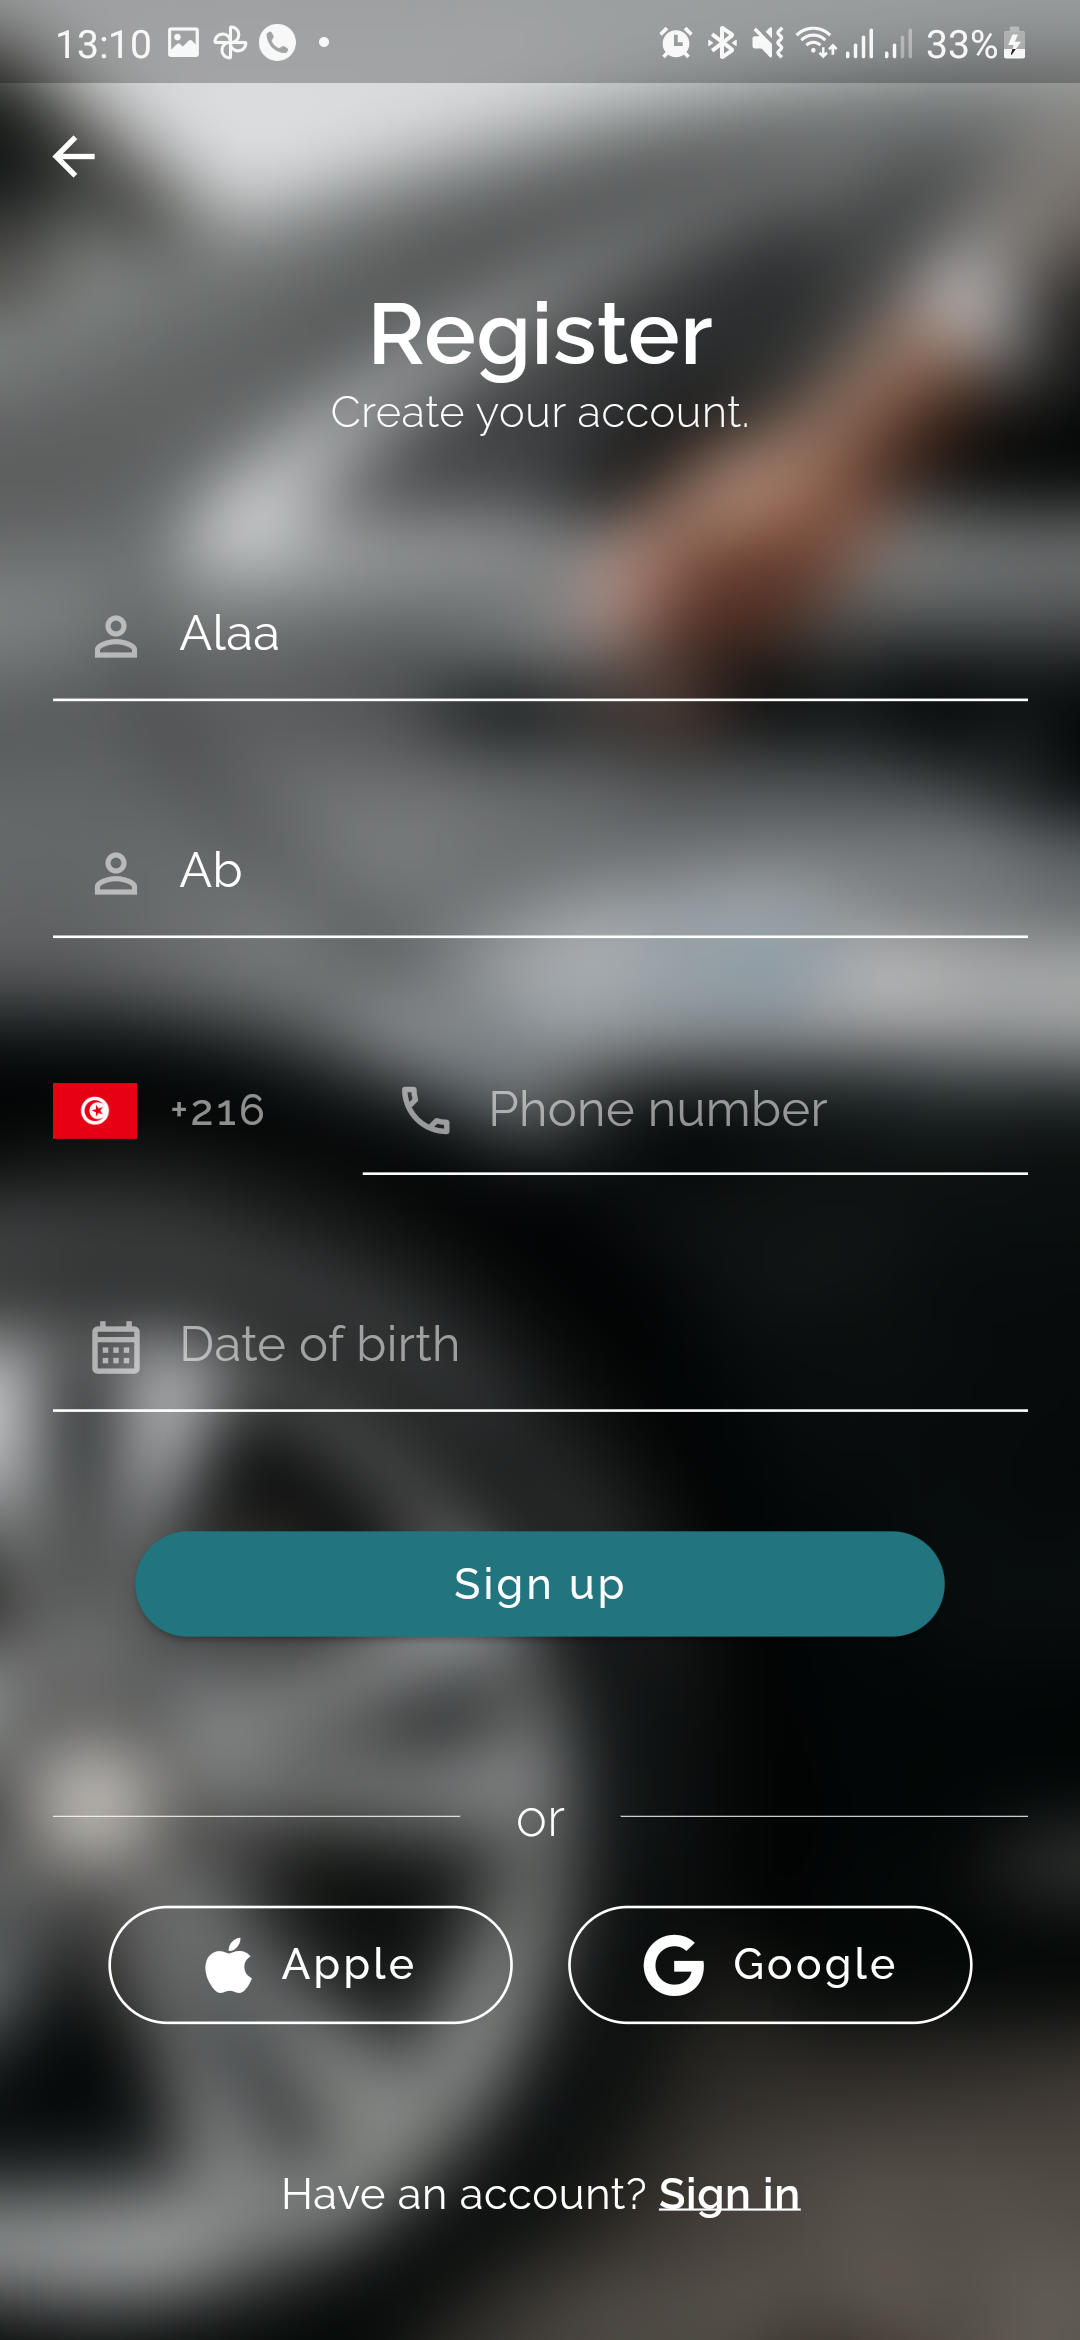
\includegraphics[height = 0.4 \textheight]{ui_screenshots/app_screenshots/finsih_register.png}
            \captionsetup{justification=centering}
            \caption{Formulaire de création de compte : 2ème étape.}
            \label{fig:app_finish_register}
        \end{center}
    \end{figure}
\end{multicols}
\subsection{Création de compte avec Google ou Apple}
Cette méthode est la plus facile et la plus rapide pour créer un compte ou s'authentifier. Avec un simple appui sur le bouton adéquat, une requête envoyée aux services de Google ou Apple pour récupérer les données du compte choisi. Ses données sont :
\begin{itemize}
    \item Un identifiant unique du compte Google ou Apple.
    \item L'adresse email du compte.
    \item Le nom et prénom utilisés avec le compte.
    \item La photo de profil utilisée avec ce compte.
\end{itemize}
Ses informations seront nécessaires pour passer la première étape de création de compte et avec eux l'utilisateur gagnera un peu de temps lors de la création de son compte.
\vspace{1cm}

\section{Authentification}
L'authentification est la première étape dans le cycle de vie de l'application, lors du premier démarrage de l'application il est nécessaire de vérifier si l'utilisateur est déjà connecté à l'application. Grâce à cette étape on peut identifier l'utilisateur, et limiter les requêtes envoyées au serveur back-end.\\
\noindent Pour s'authentifier l'utilisateur peut choisir trois méthodes différentes : Email et mot de passe, avec son compte Google, ou avec son compte Apple.\\
La validation des champs est une étape nécessaire pour s'assurer que l'utilisateur n'envoie que des valeurs correctes vers les API de connexion, ce qui permet d'éviter les erreurs inattendues.
\vspace{1cm}
\begin{center}
    \begin{multicols}{2}
        \begin{figure}[H]
            \centering
            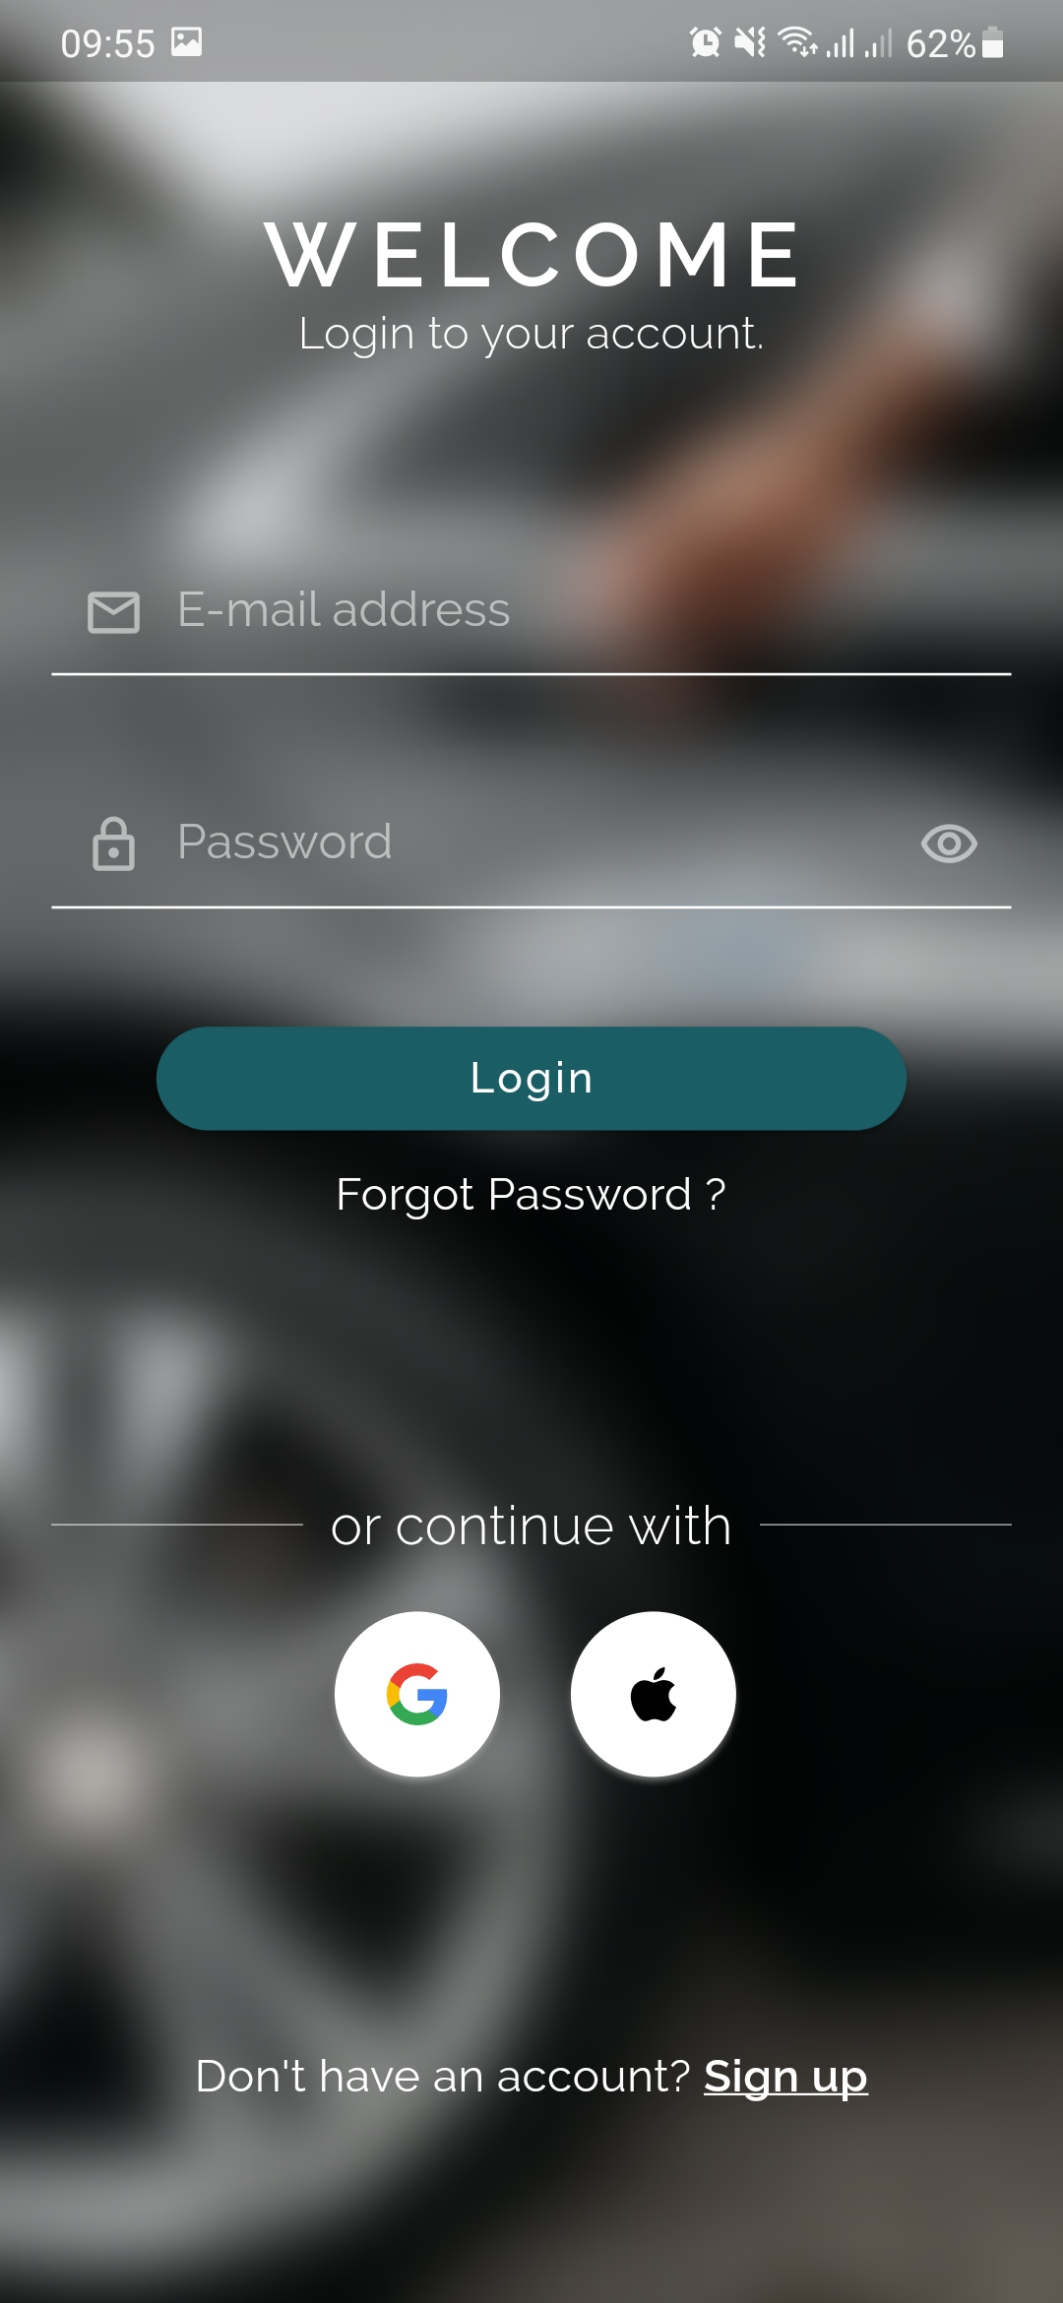
\includegraphics[height = 0.4\textheight]{ui_screenshots/app_screenshots/login_page.png}
            \vspace{1cm}
            \captionsetup{justification=centering}
            \caption{Page de Login.}
            \label{fig:app_login}
        \end{figure}
        \begin{figure}[H]
            \centering
            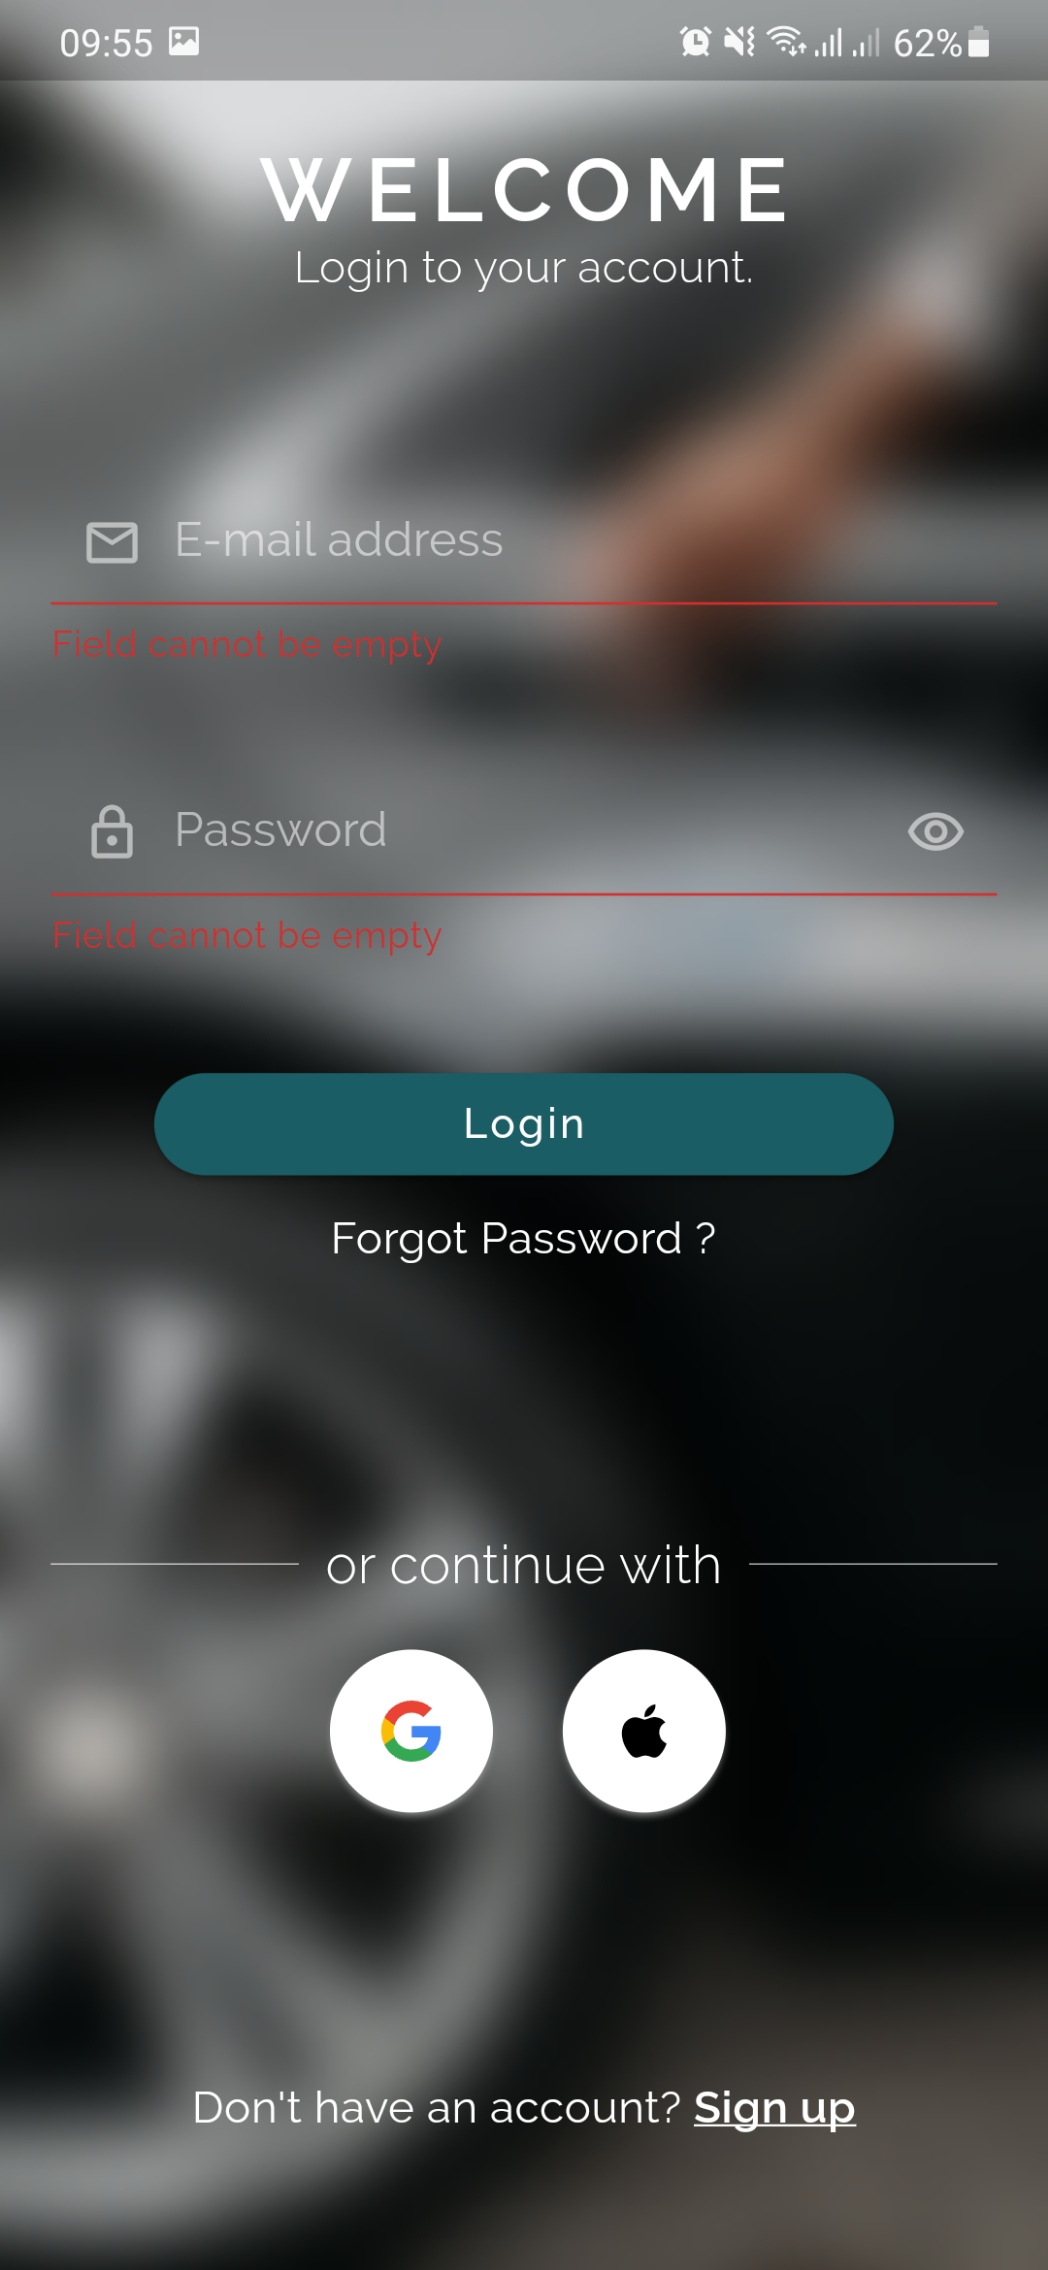
\includegraphics[height = 0.4\textheight]{ui_screenshots/app_screenshots/login_page_validation.png}
            \vspace{1cm}
            \captionsetup{justification=centering}
            \caption{Validation des champs de Login.}
            \label{fig:app_login_validation}
        \end{figure}
    \end{multicols}
\end{center}

\begin{center}
    \begin{figure}[H]
        \centering
        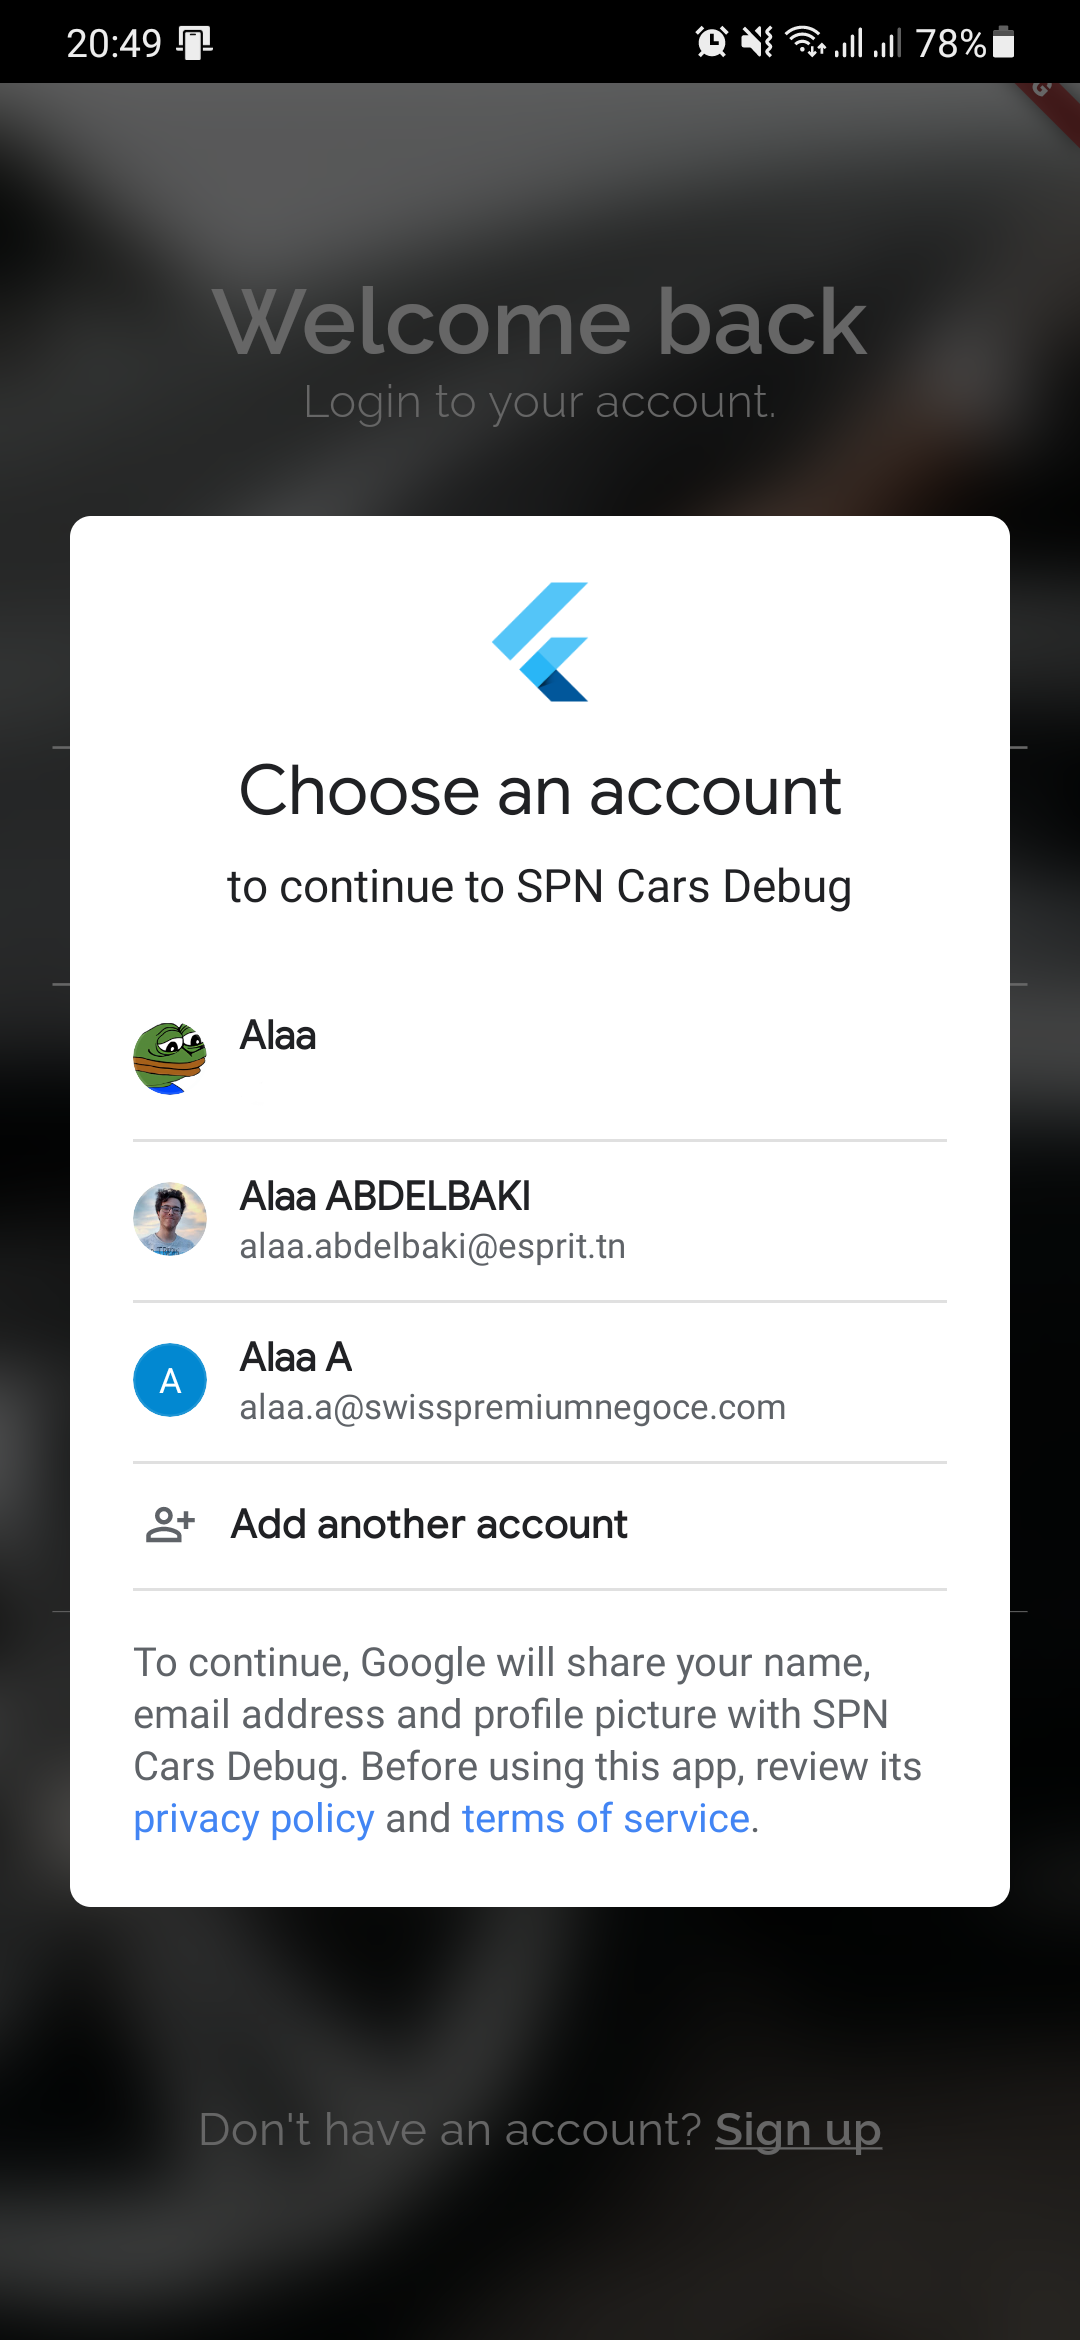
\includegraphics[height = 0.4\textheight]{ui_screenshots/app_screenshots/login_page_google.png}
        \vspace{1cm}
        \captionsetup{justification=centering}

        \caption{Login avec Google.}
        \label{fig:app_login_google}
    \end{figure}
\end{center}
\vspace{1cm}

\section{Page d'accueil}
Une fois l'utilisateur est a réussi à s'authentifier, la page d'accueil s'affiche. Cette page diffère d'un utilisateur à un autre selon les services demandés par l'utilisateur: Si l'utilisateur a un service actif le moment de sa connexion, la liste de voitures louées avec les détails de chaque service actif demandé, et s'il n'a pas de services actif le moment de sa connexion, deux boutons seront affichés : <<Rent a car>> pour louer une voiture sans chauffeur et <<Request a transfer>> pour demander un chauffeur avec une voiture.
\vspace{1cm}

\vspace{1cm}
\section{Gestion de profil}
Chaque utilisateur possède un profil personnel, ce profil affichera les informations nécessaires pour faciliter la communication entre utilisateurs dans le futur (Ex: Contact entre chauffuer et client).\\
\noindent La page de profil, dans l'application SPN-Cars, est une page très simple qui contient les informations de base de l'utilisateur :
\begin{itemize}
    \item La photo de profil.
    \item Le nom.
    \item Le prénom
    \item L'adresse E-mail.
    \item Le numéro de téléphone.
    \item La date de naissance.
\end{itemize}
De toutes ses données seuls le nom, prénom, photo de profil et numéro de téléphone seront accessibles aux chauffeurs pour assurer une communication avec les clients.\\
\noindent L'utilisateur peut modifier tous ses informations personnelles tout simplement en modifiant les champs contenant l'information à changer, et pour la photo de profile il suffit d'appuyer sur la photo pour la remplacer par une autre, soit prendre une nouvelle photo en utilisant l'appareil photo du smartphone, ou en choisissant une photo existante depuis la galerie. Une fois l'image est choisie, l'utilisateur sera redirigé vers une page pour recadrer l'image et choisir la zone qui sera affichée dans la page de profile, une fois l'image est recadrée, elle sera compressée pour réduire sa taille et faciliter son transfert vers le serveur distant.
\section{Demander un service}
Pour louer une voiture, l'utilisateur a besoin de spécifier tout d'abord les paramètres suivants :
\begin{itemize}
    \item Le type de service demandé (Location / Transfert / Excursion / Long Ride).
    \item L'adresse de départ.
    \item L'heure de départ.
    \item L'adresse d'arrivée (Pas toujours disponible selon le type de service).
    \item L'heure d'arrivée (Pas toujours disponible selon le type de service).
    \item La durée du service demandé (Pas toujours disponible selon le type de service).
\end{itemize}
\vspace{1cm}
\clearpage
\vspace{1cm}
\begin{multicols}{2}
    \begin{figure}[H]
        \centering
        \includegraphics[height = 0.4\textheight]{ui_screenshots/app_screenshots/transfer_form.png}
        \captionsetup{justification=centering}
        \caption{Formulaire de demande de transfert.}
        \label{fig:app_transfer}
    \end{figure}
    \begin{figure}[H]
        \centering
        \includegraphics[height = 0.4\textheight]{ui_screenshots/app_screenshots/current_location.png}
        \captionsetup{justification=centering}
        \caption{Utiliser le bouton <<Localiser>> pour choisir la position actuelle.}
        \label{fig:app_transfer_current_pos}
    \end{figure}
\end{multicols}
\begin{multicols}{2}
    \begin{figure}[H]
        \centering
        \includegraphics[height = 0.4\textheight]{ui_screenshots/app_screenshots/suggestions.png}
        \captionsetup{justification=centering}
        \caption{Rechercher un emplacement à l'aide de Google Places.}
        \label{fig:app_transfer_suggestions}
    \end{figure}
    \begin{figure}[H]
        \centering
        \includegraphics[height = 0.4\textheight]{ui_screenshots/app_screenshots/directions.png}
        \captionsetup{justification=centering}
        \caption{Afficher la meilleure route entre le point de départ et le point d'arrivée.}
        \label{fig:app_transfer_directions}
    \end{figure}
\end{multicols}
\section{Affichage des voitures disponibles}
Après sélection des informations nécessaires par l'utilisateur, une recherche des voitures qui répondent aux critères de recherche choisis. Une fois qu'une liste de voitures est prête, les voitures seront affichées. L'utilisateur peut appuyer sur une voiture pour découvrir ses caractéristiques et choisir ensuite de la louer ou continuer sa recherche.
\begin{multicols}{2}
    \begin{figure}[H]
        \centering
        \includegraphics[height = 0.4\textheight]{ui_screenshots/app_screenshots/available_cars.png}
        \captionsetup{justification=centering}
        \caption{Liste des voitures disponibles selon le point de départ sélectionné.}
        \label{fig:app_available_cars}
    \end{figure}
    \begin{figure}[H]
        \centering
        \includegraphics[height = 0.4\textheight]{ui_screenshots/app_screenshots/available_cars_empty.png}
        \captionsetup{justification=centering}
        \caption{Affichage si aucune voiture n'est disponible.}
        \label{fig:app_available_cars_empty}
    \end{figure}
\end{multicols}
\section{Signature numérique de contrat de location}
Pour le cas de location de voitures, un contrat doit être signé entre le client et la société. Pour s'assurer de la signature du contrat, on a opté pour la solution de signature numérique à l'aide du service offert par DocuSign, qui se spécialise dans le domaine de la signature électronique et la gestion des transactions numériques pour faciliter les échanges et les validations électroniques des contrats et de documents.\\
\noindent Pour créer une réservation de location de voitures, il suffit d'appuyer sur le bouton de <<Book now>> dans la page de détails de la voiture choisie, et une réservation sera créée avec tous les détails : La position GPS, la date de récupération et retour de voiture et les informations de contact du client. Une fois ses informations sont enregistrées, un email contenant le contrat sera envoyé au client pour le signer, et l'identifiant de ce contrat sera enregistré avec les informations de la réservation.\\
\noindent Dans l'application, le client est redirigé vers la page de vérification de signature où il doit appuyer sur le bouton de vérification de l'état de contrat. Pour signer ce contrat, il suffit d'ouvrir le document envoyé à l'adresse email du client, le signer, et retourner vers l'application. Lors de l'appui sur le bouton <<Verify Signature>>, une requête sera envoyée au back-end qui contactera les APIs de <<DocuSign>> pour vérifier l'état de signature du contrat à l'aide de l'identifiant du contrat fourni lors de la création de la réservation. Si l'état de contrat est <<sent>>, le contrat n'est pas encore signé, et un message d'erreur sera affiché à l'utilisateur. Sinon si l'état du contrat est <<completed>>, les contrat est, donc, signé et l'utilisateur est redirigé vers la page de paiement.
\vspace{1cm}

\begin{multicols}{2}
    \begin{figure}[H]
        \centering
        \includegraphics[height = 0.4\textheight]{ui_screenshots/app_screenshots/create_reservation.png}
        \captionsetup{justification=centering}
        \caption{Création de réservation.}
        \label{fig:create_res}
    \end{figure}
    \begin{figure}[H]
        \centering
        \includegraphics[height = 0.4\textheight]{ui_screenshots/app_screenshots/verify_sig.png}
        \captionsetup{justification=centering}
        \caption{Page de vérification de signature}
        \label{fig:verify_sig}
    \end{figure}
\end{multicols}
\vspace{1cm}
\clearpage
\begin{multicols}{2}
    \begin{figure}[H]
        \centering
        \includegraphics[height = 0.4\textheight]{ui_screenshots/app_screenshots/not_signed.png}
        \captionsetup{justification=centering}
        \caption{Vérification de signature avec un document non signé.}
        \label{fig:not_signed}
    \end{figure}
    \begin{figure}[H]
        \centering
        \includegraphics[height = 0.4\textheight]{ui_screenshots/app_screenshots/contract_email.png}
        \captionsetup{justification=centering}
        \caption{Email contenant les documents à signer.}
        \label{fig:sign_documents}
    \end{figure}
\end{multicols}
\vspace{1cm}
\begin{multicols}{2}
    \begin{figure}[H]
        \centering
        \includegraphics[height = 0.4\textheight]{ui_screenshots/app_screenshots/signature.png}
        \captionsetup{justification=centering}
        \caption{Choix de signature.}
        \label{fig:signature_select}
    \end{figure}
    \begin{figure}[H]
        \centering
        \includegraphics[height = 0.4\textheight]{ui_screenshots/app_screenshots/signature_end.png}
        \captionsetup{justification=centering}
        \caption{confirmation de signature.}
        \label{fig:confirm_sig}
    \end{figure}
\end{multicols}
\section{Paiement}
Pour le paiement des services offerts par SPN Cars, l'utilisateur utilisera <<Apple Pay>> s'il utilise un iPhone ou <<Google Pay>> s'il utilise un smartphone Android, qui sont, grâce à leurs haute disponibilités, le choix optimal pour effectuer des paiements en ligne avec son propre smartphone.\\
Pour effectuer un paiement avec l'application SPN Cars, il suffit de signer le contrat de location dans le cas de location de voitures, ou sélectionner une voiture dans le cas de demande de transfert, après la page de paiement avec le bouton de paiement selon le type de smartphone sera affiché. Lors de l'appui, L'interface des applications de paiement adéquates sera affichée pour continuer la transaction. Une fois terminé, l'utilisateur sera redirigé vers la page d'accueil si le paiement est effectué, ou un message d'erreur sera affiché si non.
\vspace{1cm}

\begin{multicols}{2}
    \begin{figure}[H]
        \centering
        \includegraphics[height = 0.4\textheight]{ui_screenshots/app_screenshots/checkout.png}
        \captionsetup{justification=centering}
        \caption{Interface de paiement.}
        \label{fig:checkout}
    \end{figure}
    \begin{figure}[H]
        \centering
        \includegraphics[height = 0.4\textheight]{ui_screenshots/app_screenshots/pay_details.png}
        \captionsetup{justification=centering}
        \caption{Détails de paiement.}
        \label{fig:pay_details}
    \end{figure}
\end{multicols}
\section{Localiser une voiture}
Lorsqu'une réservation atteint la date de début et sera affichée dans la page d'accueil, le client peut appuyer sur la réservation et voir plus de détails sur sa réservation et sa voiture. Une fois appuyé sur le bouton <<See more>>, le client sera redériger vers une page qui affiche la position de sa voiture sur un plan. Cette position sera mise à jour en temps réel si le chauffeur est en train de conduire la voiture.\\
\noindent La page permet aussi d'afficher les informations basiques du chauffeur avec une possibilité de le contacter soit par appel téléphonique soit par message.
\begin{figure}[H]
    \centering
    \includegraphics[height= 0.4\textheight]{ui_screenshots/app_screenshots/details.png}
    \captionsetup{justification=centering}
    \caption{Affichage des détails de la réservation.}
    \label{fig:res_details}
\end{figure}
\section{Messagerie instantanée}
Une fois que l'utilisateur a appuyé sur le bouton pour contacter le chauffeur par messagerie instantanée, l'utilisateur est redirigé vers une page de messagerie avec le chauffeur où ils peuvent échanger des messages.\\
\noindent L'utilisateur peut aussi retourner vers sa liste de conversations et afficher ses anciens messages depuis la page d'accueil.
\clearpage
\begin{multicols}{2}
    \begin{figure}[H]
        \centering
        \includegraphics[height = 0.4\textheight]{ui_screenshots/app_screenshots/messages_list.png}
        \vspace{1cm}
        \captionsetup{justification=centering}
        \caption{Liste de messages de l'utilisateur.}
        \label{fig:message_list}
    \end{figure}
    \begin{figure}[H]
        \centering
        \includegraphics[height = 0.4\textheight]{ui_screenshots/app_screenshots/messages_details.png}
        \vspace{1cm}
        \captionsetup{justification=centering}
        \caption{Conversation avec l'utilisateur.}
        \label{fig:conversation}
    \end{figure}
\end{multicols}
\section{Documentation des API}
La documentation des APIs est une étape nécessaire dans le développement de n'importe quelle application. Une documentation accessible et facilement exploitable est une condition préalable au développement des API. Il est important d'avoir une documentation toujours à jour quand le code/les fonctionnalités de l'API évoluent.\\
\noindent Et puisque le modèle de développement chez SPN est centré sur le travail collaboratif, il est très important d'avoir une documentation claire et et facile à exploiter des APIs.

On va prendre un exemple de documentation de l'API de l'entitée <<Voiture>> où on a suivi les spécifications de Open Api pour créer la documentation de ses APIs.
\begin{figure}[H]
    \centering
    \includegraphics[height= \textheight]{openapi.png}
    \captionsetup{justification=centering}
    \caption{Schéma de documentation des API.}
    \label{fig:api_doc_schema}
\end{figure}
\newpage
\begin{figure}[H]
    \centering
    \includegraphics[height= 0.8\textheight,width=\textwidth]{api.png}
    \captionsetup{justification=centering}
    \caption{Documentation des API.}
    \label{fig:api_doc}
\end{figure}
\begin{figure}[H]
    \centering
    \includegraphics[height= 0.8\textheight,width=\textwidth]{add_car.png}
    \captionsetup{justification=centering}
    \caption{Détails API ajout voiture.}
    \label{fig:api_doc_detail}
\end{figure}
\clearpage
\section{Conclusion}
Dans ce chapitre on a présenté la réalisation de l'application, où on a décrit chaque fonctionnalité de l'application avec des captures d'écran qui montrent les différentes interfaces. On a commencé par l'étape de création de compte et connexion qui permettra au client d'utiliser les différents services offerts par l'application et on a passé par les différentes fonctionnalités une par une.\\
\noindent On a présenté aussi l'étape de documentation des APIs qui permettra de faciliter la collaboration avec d'autres équipes et l'amélioration de leur fonctionnement dans le futur.
\newpage
\chapter*{Conclusion générale}
\markboth{CONCLUSION GÉNÉRALE}{CONCLUSION GÉNÉRALE} %
\addcontentsline{toc}{chapter}{Conclusion générale}
\vspace{1cm}
\justifying
\lettrine[findent=2pt,lines=3]{\textit{D}}{}ans le présent rapport, on a dressé le bilan complet de ce travail qui se situe dans le cadre de mon projet de fin d'études. L'objectif principal de ce projet étant de concevoir et de développer une application mobile de location de voitures de luxes pour les clients de Swiss Premium Negoce, l'entreprise acceuillante.

On a entamé ce rapport par une présentation du cadre général du projet où on a présenté l'entreprise acceuillante et ses activitées, puis on a présenté des différentes applications qui offrent des services de location de voitures et service taxi, ses applications on présenté des inconvénients. On a dégagé d'après ses inconvénients la problématique ayant engendré le besoin d'unne telle application. Pour réaliser cette application, on a dû ensuite séparer ses boisoins en besoins fonctionnels et non fonctionnels qui ont permis de commencer l'étape de conception, où on a décrit les différentes fonctionnalités nécessaires. Cette étape a permis d'identifier les technologies et outils à utiliser pour arriver à réaliser ce projet dans les délais choisis.\\
\noindent Une fois les outils et technologies choisies, on a passé au développement de l'application, où on a commencé par le développement des interfaces graphiques avec Flutter et leurs fonctionnalités avec Javascript et ExpressJS en coté serveur, au fin de développement de chaque interface et ses fonctionnalités, elle est testée pour dégager les différentes erreurs qui peuvent se déclancher et les corriger, jusqu'au développement de la dernière interface de l'application.

Ce projet fut une expérience enrichissante et fructueuse qui m'a permis d'acquérir de nouvelles compétences de grande valeur dans plusieurs domaines à la fois : Le développement web, davelopmmenet mobile et le design des interfaces graphique et l'expérience utilisateur (UI/UX Design), en particulier le développement des applications coté serveur avec ExpressJS, développement des applications mobiles avec Flutter et la création des maquettes des interfaces utilisateur avec Adobe XD. Ainsi, ce stage qui représente une nouvelle expérience professionnelle, m'a été bénéfique, il a été une nouvelle chance pour consolider mes compétences techniques et mettre en pratique mes compétences théoriques.

J'ai appris à être autonome, ouvert aux autres, et plus conscient de la vie professionnelle qui nécessite la ponctualité, le sérieux et le travail acharné. J'ai pris la responsabilité et j'ai développé l'application qui répondait aux besoins définis dans le cahier de charges, les exigences, et les délais.

Comme tout projet informatique, des contraints on été rencontrées et elles ont été surmontées tout au long de la réalisation du projet. Elles ont constitué un défi pour acquérir de nouvekkes connaissances techniques et de développer les capacités opérationnelles. Ces défis concernent notamment la familiarisation avec les nouveaux frameworks et la maîtrise de certains outils techniques.

J'espère que le présent rapport soit suffisamment clair et structuré pour sue le lecteur ait une idée précise et complète sur les différentes tâches que j'ai effectuées.

\newpage
\includepdf[pages={1}]{./chapters/last.pdf}

\end{document}
